%% The '3p' and 'times' class options of elsarticle are used for Elsevier CRC
%% Add the 'procedia' option to approximate to the Word template
%\documentclass[3p,times,procedia]{elsarticle}
\documentclass[3p,times]{elsarticle}

%% The `ecrc' package must be called to make the CRC functionality available
\usepackage{ecrc}

%% The ecrc package defines commands needed for running heads and logos.
%% For running heads, you can set the journal name, the volume, the starting page and the authors

%% set the volume if you know. Otherwise `00'
\volume{00}

%% set the starting page if not 1
\firstpage{1}

%% Give the name of the journal
\journalname{Journal of Parallel and Distributed Computing}

%% Give the author list to appear in the running head
%% Example \runauth{C.V. Radhakrishnan et al.}
\runauth{P. Li et al.}

%% The choice of journal logo is determined by the \jid and \jnltitlelogo commands.
%% A user-supplied logo with the name <\jid>logo.pdf will be inserted if present.
%% e.g. if \jid{yspmi} the system will look for a file yspmilogo.pdf
%% Otherwise the content of \jnltitlelogo will be set between horizontal lines as a default logo

%% Give the abbreviation of the Journal.  Contact the journal editorial office if in any doubt
\jid{procs}

%% Give a short journal name for the dummy logo (if needed)
\jnltitlelogo{J. Parallel Distrib. Comput.}

%% Provide the copyright line to appear in the abstract
%% Usage:
%   \CopyrightLine[<text-before-year>]{<year>}{<restt-of-the-copyright-text>}
%   \CopyrightLine[Crown copyright]{2011}{Published by Elsevier Ltd.}
%   \CopyrightLine{2011}{Elsevier Ltd. All rights reserved}
\CopyrightLine{2014}{Published by Elsevier Ltd.}

%% Hereafter the template follows `elsarticle'.
%% For more details see the existing template files elsarticle-template-harv.tex and elsarticle-template-num.tex.

%% Elsevier CRC generally uses a numbered reference style
%% For this, the conventions of elsarticle-template-num.tex should be followed (included below)
%% If using BibTeX, use the style file elsarticle-num.bst

%% End of ecrc-specific commands
%%%%%%%%%%%%%%%%%%%%%%%%%%%%%%%%%%%%%%%%%%%%%%%%%%%%%%%%%%%%%%%%%%%%%%%%%%

%% The amssymb package provides various useful mathematical symbols
\usepackage{amssymb}
%% The amsthm package provides extended theorem environments
%% \usepackage{amsthm}

%% The lineno packages adds line numbers. Start line numbering with
%% \begin{linenumbers}, end it with \end{linenumbers}. Or switch it on
%% for the whole article with \linenumbers after \end{frontmatter}.
%% \usepackage{lineno}

%% natbib.sty is loaded by default. However, natbib options can be
%% provided with \biboptions{...} command. Following options are
%% valid:

%%   round  -  round parentheses are used (default)
%%   square -  square brackets are used   [option]
%%   curly  -  curly braces are used      {option}
%%   angle  -  angle brackets are used    <option>
%%   semicolon  -  multiple citations separated by semi-colon
%%   colon  - same as semicolon, an earlier confusion
%%   comma  -  separated by comma
%%   numbers-  selects numerical citations
%%   super  -  numerical citations as superscripts
%%   sort   -  sorts multiple citations according to order in ref. list
%%   sort&compress   -  like sort, but also compresses numerical citations
%%   compress - compresses without sorting
%%
%% \biboptions{comma,round}

% \biboptions{}

% if you have landscape tables
\usepackage[figuresright]{rotating}

% put your own definitions here:
%   \newcommand{\cZ}{\cal{Z}}
%   \newtheorem{def}{Definition}[section]
%   ...


\usepackage{psfig}
\usepackage{graphicx}
\usepackage{textcomp}
\usepackage{amsmath}
\usepackage{amssymb}
\usepackage{longtable}
\usepackage{array}
\usepackage{algorithm}
\usepackage{algorithmic}
\usepackage{color}
\newcommand{\reminder}[1]{{{\textcolor{blue}{\bf (#1)}}}}
\newcommand{\tabincell}[2]{\begin{tabular}{@{}#1@{}}#2\end{tabular}}
\usepackage{url}



%-------------------------------------------------------------------------
% take the % away on next line to produce the final camera-ready version
%\pagestyle{empty}

%-------------------------------------------------------------------------
\begin{document}

\begin{frontmatter}

\title{Transformer: Run-time Reprogrammable Heterogeneous Architecture
  for Transparent Acceleration of Dynamic Workloads}


\author{Peilong Li}
\ead{Peilong\_Li@student.uml.edu}
\author{Yan Luo}
\address{University of Massachusetts Lowell, One University Ave, Lowell, MA, USA, 01854}
\author{Jun Yang}
\address{University of Pittsburgh, 4200 Fifth Avenue, Pittsburgh, PA, USA, 15260}

\begin{abstract}

Heterogeneous architectures face challenges on resource allocation to
cores and accelerators as well as transparent acceleration.  We
propose "{\em Transformer}", a run-time reprogrammable, heterogeneous
architecture with cores and reconfigurable logics for supporting
coarse-grained acceleration of dynamic, unpredictable workloads
presented in mobile and cloud computing environments. The architecture
allows run-time instantiation of one or more acceleration functions in
an on-chip reconfigurable logic in response to the demands of
compute-intensive software libraries. We design a hardware controller
and software wrapper functions to profile workloads, reprogram the
logic and invoke accelerators. Novel heuristics are derived to
schedule accelerator functions. We explore the optimal chip resource
allocation for cores and accelerators. Our simulation results show
that Transformer brings significant improvement on both performance
(up to 14x for single-type workloads and up to 2.3x for dynamic
workloads) and energy efficiency (up to 6.9x) for a wide range of
workloads.

\end{abstract}


\begin{keyword}
Accelerator \sep Transparent acceleration \sep Coarse-grain
\sep Heterogeneous architecture \sep FPGA
%% keywords here, in the form: keyword \sep keyword

%% PACS codes here, in the form: \PACS code \sep code

%% MSC codes here, in the form: \MSC code \sep code
%% or \MSC[2008] code \sep code (2000 is the default)

\end{keyword}

\end{frontmatter}


\section{Introduction}


Chip Multi-Processors (CMPs) have become the mainstream processors for
mobile, desktop and cloud computing platforms due to the power
budget and the limits on clock frequency scaling. While
thread-level parallelism can be well leveraged with CMPs \cite{CMP05}
for throughput oriented applications, the single-thread performance of
a processor remains important to time critical workloads. For this
reason it is common to integrate various ASIC-based special 
purpose accelerators with general purpose cores into
a system-on-chip (SoC) heterogeneous processor
\cite{soc-acc} to improve its single-thread performance. 

However, ASIC based on-chip accelerators do not respond well to
emerging dynamic workloads where applications come and go either on
demand or in a unpredictable manner. For example, a smartphone can
support an exponentially growing number of Apps in social, gaming,
health, location and other domains. The user of a smartphone may
install or uninstall Apps at any time, leading to a changing mixture
of applications. A cloud computing platform such as Amazon EC2
\cite{amazon-ec2} executes various workloads such as Web
\cite{Chen:2012jo}, data mining \cite{ec2-datamining}, DNA sequencing
\cite{ec2-dna} submitted from users' Virtual Machines (VMs) at
arbitrary moments. Even though SoCs with built-in accelerators are
optimized for a fixed set of common functions such as encryption and
compression, these functions may not be needed at certain time periods
or for a given workload mix. As a result, such fixed accelerators
become dormant for a prolonged time span, wasting silicon resources.

A complementing approach is to use off-chip programmable hardware
accelerators like GPU and FPGA to speed up complex workloads
\cite{GPUFPGA, fpga-acc}. However, such hardware acceleration units do
not meet the stringent time requirements of delay-sensitive workloads
due to conventional system architectures. These units are typically
connected to the processor cores via off-chip interconnects
(e.g. PCIe, QPI \cite{intel-qpi} or HyperTransport
\cite{amd-hypertransport}) with serious latency limits, resulting
significant delays in data transfer. Thus, even with massively
parallel processing capabilities, FPGAs and GPUs are challenged to
deliver the expected speedup in reality. Their performance advantages
and flexibility in reprogramming cannot be harnessed to the full
extent until an architectural change occurs on their interconnects to
cores.
%among programmable accelerators and general purpose cores happens.

Leveraging on-chip accelerators in existing and new applications is
not trivial as redevelopment cost is prohibitive.  Allowing an
applications' execution flow transparently directed to accelerators
without any user intervention remains an interesting but unsolved
issue. As new instructions are typically added along with SoC
accelerators, rewriting and recompiling an application's code is
mandatory. Fine-grained accelerations such as
\cite{Govindaraju:2012fn} also require compiler support. Since IPs for
FPGAs and programs developed for GPUs keep increasing, it makes sense
to incorporate them through coarse-grained acceleration, i.e. the
speedup of an entire function (e.g. 3DES encryption) as an element of
an existing software library (e.g. libopenssl). Such library based
approach facilitates acceleration without incurring (re)development
costs for users.

The power efficiency \cite{hamada09,thomas09} and performance benefits
of recent programmable hardware have been driving the momentum of
heterogeneous computing platforms that combine general-purpose cores
and reconfigurable logics (e.g. Convey HC-1 \cite{brewer09} and Cray
XD1\cite{Ulmer:2005vh}) for high performance computing (HPC)
applications. However, the workloads in many computing environments
are far more dynamic and versatile than those in HPC domain. The
fusion of general-purpose cores and programmable logics for
power-efficient computing is inadequately investigated in terms of
architecture trade-offs on performance and power, transparent
acceleration, and accelerator-aware scheduling, all of which are
critical to the practical deployment of programmable heterogeneous
architectures.

We propose {\em Transformer}, a heterogeneous architecture with both
general purpose cores and on-chip programmable accelerator logics for
addressing the challenges introduced by dynamic workloads in many
emerging scenarios. This architecture differs from existing works in
several aspects: (1) the architecture consists of on-chip programmable
accelerators with general purpose cores.  Sharing the memory hierarchy
with cores, the accelerators are promoted to first-class citizens and
access cores' data in an efficient way to reduce latency;  
%The
%proximity of cores and programmable accelerators promote the
%accelerators to first class citizens of the system, eliminating the
%overheads of off-chip communications; 
(2) sharing an accelerator unit among multiple acceleration functions
improves the utilization of the chip resources. Optimal area resource
allocation to cores and accelerators leads to improved performance and
energy efficiency. Our proposed heuristics maximize the memory
bandwidth utilization and improve speedup of unpredictable workload
mixtures under given resource constraints; and (3) the architecture
enables transparent acceleration with novel middleware support,
significantly reducing deployment costs.  It is worth noting that,
while the programmable accelerator logics in the proposed architecture
can be GPU based coprocessors \cite{intel-gpu}, we focus in this paper
on FPGA-type reconfigurable logics due to the large set of existing IP
designs available for FPGAs and their improved power
efficiency. Nevertheless the middleware and scheduling algorithms
studied in this research are generic enough for benefiting either
implementation.

We make the following contributions in this work:
\begin{enumerate}

\item We present a deployable heterogeneous architecture with run-time
  programmable on-chip accelerators. Our study evaluates the
  performance benefits of on-demand accelerators, and explores the
  design space of silicon resource allocation to cores and
  accelerators.

\item We design a suite of middleware and scheduling algorithm for
  supporting transparent acceleration, which is an enabling factor for
  the wide deployment of accelerators, but not explicitly addressed in
  prior research. To the best of our knowledge, our work is the first
  to address this issue and present a viable solution.

\item We characterize the power consumption of the proposed
  heterogeneous architecture with industrial level power modeling
  tools. This study gives important insights on the scalability and
  power-performance trade-offs.

\end{enumerate}

The paper is organized as follows. Section \ref{sec_related} discusses
prior work related to our research. Section \ref{sec_arch} describes
the proposed programmable heterogeneous architecture, followed by the
transparent acceleration mechanisms detailed in Section
\ref{sec_transacc}. We present the accelerator-aware scheduling and
accelerator combination algorithms in Section
\ref{sec_runtime_reconfig}. Performance evaluation methodology and
experiment results are presented in Section \ref{sec_perf}. Finally we
conclude the paper in Section \ref{sec_concl}.

 \if 0 FPGA as a
co-processing unit, has demonstrated the ability to speed up a variety
of applications, such as image processing \cite{imageacc}, data mining
\cite{data-mining-ref}, bioinformatics \cite{bioacc1} \cite{bioacc2},
navigation \cite{naviacc} and encryption/decryption
\cite{encryptionacc}. As another popular alternative acceleration
method, GPGPUs are less expensive and have higher memory bandwidth and
a larger number of programmable cores with thousands of hardware
threads than FPGA. So if the data to be processed can be simply
divided into many parallel trunks without any dependency or shared
data, it can be easily processed though the GPU
optimizations. However, there are several limitations of GPU that may
severely affect the computing performance on threaded GPU
platform. First, it is usually difficult to find how much data
parallelism lies in the application because no aspects of GPUs are
transparent to programmers \cite{microsoft06}. Second, scatter and
gather are two basic operations performed by GPU, which will also
introduce a gigantic amount of memory access latency and degradation
of memory bandwidth because of their access randomness
\cite{GPUlimit1}. Third, there are many domains of application with
large data dependency that are not optimized well on GPU
\cite{GPUlimit2}.  \fi


\section{Related Work}
\label{sec_related}
Cong et al. \cite{accrich,cong-islped12,cong-saw11} propose a
heterogeneous architecture called CHARM with loosely-coupled on-chip
accelerators. By composing the accelerator building blocks, the
architecture can dynamically speed up medical imaging benchmarks (up
to 3.7x) and show energy consumption reduction by up to 4.7x.  In
spite of its effectiveness in computation acceleration, this
accelerator-rich architecture introduces new accelerator instructions and
requires recompiling applications, lacking the run-time
reconfigurability.  Garcia et al. propose software based kernel sharing in a
multiprocessor system with reconfigurable hardware
	\cite{Garcia:2008iy}. This concept is similar with CHARM as both
of them emphasize the strategies on how to best utilize the existing
accelerator.

Our work differs from CHARM \cite{accrich,cong-islped12,cong-saw11} as
follows: (a) Transformer is targeted at cloud and mobile applications
where the execution environment has to handle dynamics of the
workloads as they arrive and depart at unpredictable time. So
Transformer focuses on run-time profiling workloads and reprogramming
acceleration functions accordingly. CHARM, on the other hand,
emphasizes on sharing the existing accelerators among software
threads, lacking the ability of coping with emerging workloads at
run-time; (b) Transformer incorporates a centralized reconfigurable
logic, instead of distributed fine-grained accelerator blocks in other works 
\cite{accrich}, to improve the area utilization. The chip
resource dedicated to the acceleration logic can be re-programmed and
shared by multiple accelerator engines for different functions, thanks
to the partial reconfiguration technology.  We develop heuristics to
combining accelerators on-demand for maximizing memory bandwidth
utilization or speedup effect; and (c) Transformer has a set of
middleware innovations that avoid rewriting user applications with a
library-oriented coarse-grained approach. This is supported by the
growing set of available soft IP cores for reconfigurable logic
\cite{opencores,design-reuse,free-ip}. In contrast, CHARM requires
rewriting user code.

Govindaraju et al. propose {\em DySER} with both functionality and
data parallelism specialization \cite{Govindaraju:2012fn,Govindaraju:HPCA11}. DySER
provides the feasibility of dynamically specializing execution
resources and creating various data path for parallelizable
``hot-spot'' in workload, and thus improve the performance and energy
efficiency. {\em Transformer}, in another research direction, aims at
coarse-grained acceleration at the level of a library function. {\em
  DySER} relies on a compiler to partition hot spots into compute and
data subregions and offload to dynamically formed functional
units. Without compiler assistance, {\em Transformer} contains
hardware and middleware to perform run-time reconfiguration to avoid
recompilation, supporting the acceleration of closed-source
executables.

{\em Garp} \cite{Garp:1997,Garp:2000} and {\em Transformer} target on
the same direction: that is, improving computation performance and power
efficiency with FPGA-based parallelization. However, the two
architectures focus on different granularities of parallelism. Similar
to {\em DySER}, {\em Garp} targets on a finer granularity with the
optimization of basic operations to achieve instruction level
parallelism. Such parallelization heavily relies on a compiler because the compiler needs to
precisely identify the potential parallelizable code and map the code
to an acceleration block in a way that its performance could be
improved. The penalty of imprecise identification is significant at such instruction level granularity.
%Otherwise, the compiler optimized code might compromise the
%performance. 
Our approach focuses on the optimization at library (function) level,
considering the data sharing and computation in a global
view, so it usually guarantees performance improvement. We always know
an optimized version on FPGA outperforms the CPU version of the same
function with tens or even hundreds of speedup. We just need to make
sure to plug in the right accelerator at the right time to tackle with
the dynamics of the workload. The profiling and scheduling methods are applicable to fine-granularity acceleration too.

Other works such as HiPPAI \cite{Stillwell:2009if} and EXOCHI
\cite{Wang:2007bc} propose new programming environment or interface
for hardware accelerated SoC platform. HiPPAI abstracts a layer of
accelerator interface in OS to schedule task either onto the
accelerator or to the general purpose core. However, this layer of
abstraction lacks the awareness of the run-time dynamics on the
accelerator. In contrast, we propose a reconfiguration controller to
keep track of the usage information on logic and make 
efficient use of the logic resource, without requiring reprogramming. 

Towards high performance big data applications, LINQits is proposed as
a flexible hardware template that can be mapped onto programmable
logic or ASICs in a heterogeneous system-on-chip for a mobile device
or a server \cite{Chung:2013:LBD:2485922.2485945}. LINQits accelerates a domain-specific query
language called LINQ, and LINQits requires applications (re-)written with
LINQ for taking advantage of hardware acceleration. 

While the LINQits architecture has similarities with our proposed {\em
  Transformer} architecture in a ``core + FPGA'' form, there exist
notable differences between them: (a) {\em Transformer} is a
generic architecture not tied to a particular application domain
whereas LINQits is designed and optimized for big data applications; 
and (b) no rewriting or recompiling application is needed in {\em Transformer} while
LINQits relies on rewriting applications with LINQ language
constructs, which are not applicable for non-database applications.

Huang et al. propose an aggregate gain algorithm (AG)
\cite{Huang:2009hs} to predict future acceleration requirement of the
workload. This prediction mechanism may work properly on some specific
domain of computing, however, cloud workloads are too dynamic to be
accurately predicted. Also in Huang's work, cache coherency is not considered and the
number of LUTs is the only resource constraint. {\em Transformer}
maintains coherency on both cores' caches and accelerators' local
memory and considers constraints of all logic resources (LUT, BRAM,
SLICE, etc.).


Mignolet et al. \cite{Mignolet:2003gr} introduce a feasible way of
relocating tasks between software path and accelerated hardware
path. They implement a new OS (OS4RS) which contains a hardware
abstraction layer and a communication interface to enable OS tasking
scheduling between software and hardware. 
However, {\em Transformer} does not require changes to OS
layer. Instead, transparent acceleration in {\em Transformer} is
achieved with a wrapper library which resides at the middleware layer,
improving the portability of the design.


Supercomputers pursue the highest computation performance
\cite{Ulmer:2005vh} with supports of FPGAs. For instance, each node
(six nodes in a chassis) in Cray XD1 integrates one Xilinx Virtex-4
connected via a RadipArray Interconnect to four memory banks shared
with two AMD Opteron processors. Though both providing run-time
reprogrammability, Cray XD1 differs from {\em Transformer} in two
aspects: (a) reconfigurable logic on Cray XD1 is an off-chip
coprocessor which communicates with CPUs under the control of Rapid
Array Processors whereas {\em Transformer} integrates reconfigurable
logic onto the SoC, permitting on-chip data sharing with cores and (b)
to utilize the coprocessors on Cray XD1, users need to apply the
vendor-provided FPGA Linux API into their software design. In
contrast, {\em Transformer} provides a transparent scheme of invoking
accelerators.

As an ``extreme" form on fixed specialization, conservation cores
\cite{Venkatesh:2010:CCR:1735970.1736044,Venkatesh:2010:CCR:1736020.1736044,Venkatesh:2010:CCR:1735971.1736044},
or c-cores, are specialized processors that focus only on energy and
energy-delay efficiency rather than improving performance. C-cores
provides a promising reduction of energy consumption (up to
16.0$\times$ for specific functions and up to 2.1$\times$ for whole
application), which is comparable with {\em Transformer}'s energy
efficiency (up to 6.9$\times$), at the risk of compromising the
performance. However, we argue that QoS is one of the most important
concerns for most of the cloud service provider, that is, providing
the best user experience. Thus, the balance between performance and
power consumption should be carefully considered. {\em Transformer}
provides a solution that considers both performance and power aspects
in cloud services. In addition, the service provider typically does
not have access to the source code used or owned by the customers in a
cloud computing environment. This makes c-core ineffective in such scenarios. {\em Transformer}'s middleware approach based on wrapper library imposes no requirements on source code access, therefore is feasible for a wide range of applications. 

Given the reprogramming/partial-reconfiguration costs of FPGA-type of
logic (in the order of tens or hundreds of milliseconds depending on
the size of bit streams \cite{Liu:2009ie}), the benefits of adapting
the accelerator functions at run-time must outweigh such
costs. Characterization on cloud computing workloads has demonstrated that the lifetime of various
applications ranges from 300 to 86400 seconds \cite{CloudWorkload}, implying that an
accelerated function would be used for a considerable duration. This
validates our rationale of reprogramming accelerators with different
functions on-demand.

Our proposed architecture is built atop of partial reconfiguration
technology such as XILINX Dynamic Partial Reconfiguration (DPR)
\cite{PRUserGuide} to reduce reconfiguration time while not
interrupting the operation of other logic. For example, in Xilinx DPR
design process, a library of hardware modules called Partially
Reconfigurable Modules (PRMs) and their corresponding Partial Bit
Streams (PBS) are created in advance. 
%The circuits that are not configurable during runtime are called Static Region. 
During runtime, PBSs are configured to a region on device called
Partial Reconfigurable Region (PRR) through a primitive configuration
module known as Internal Configuration Access Port (ICAP)
\cite{Hansen:2011dt,Liu:2009ie,McDonald:2008ec}. We leverage ICAP-like
structure to reprogram the configurable logic on demand.





\section{Transformer - Run-time Reconfigurable Heterogeneous Architecture}
\label{sec_arch}


\subsection{Architecture Overview}

Figure \ref{fig_arch} shows {\em Transformer}, heterogeneous
architecture for transparent acceleration of dynamic
workloads. Transformer consists of cores with private L1 caches, and a
partial reconfigurable logic unit ( also called programmable
accelerator in this paper) for instantiating acceleration
functions. The reconfigurable logic, equipped with input and output
buffers, shares the L2 cache with the cores through dedicated DMA
channels. All processing elements (cores and accelerator) are
interconnected via a mesh-type network on chip (NoC). The memory
hierarchy (private memory units of both cores and the accelerator,
shared L2 cache and main memory) follows MOESI protocol to maintain
coherence.

\begin{figure}
    \centering
    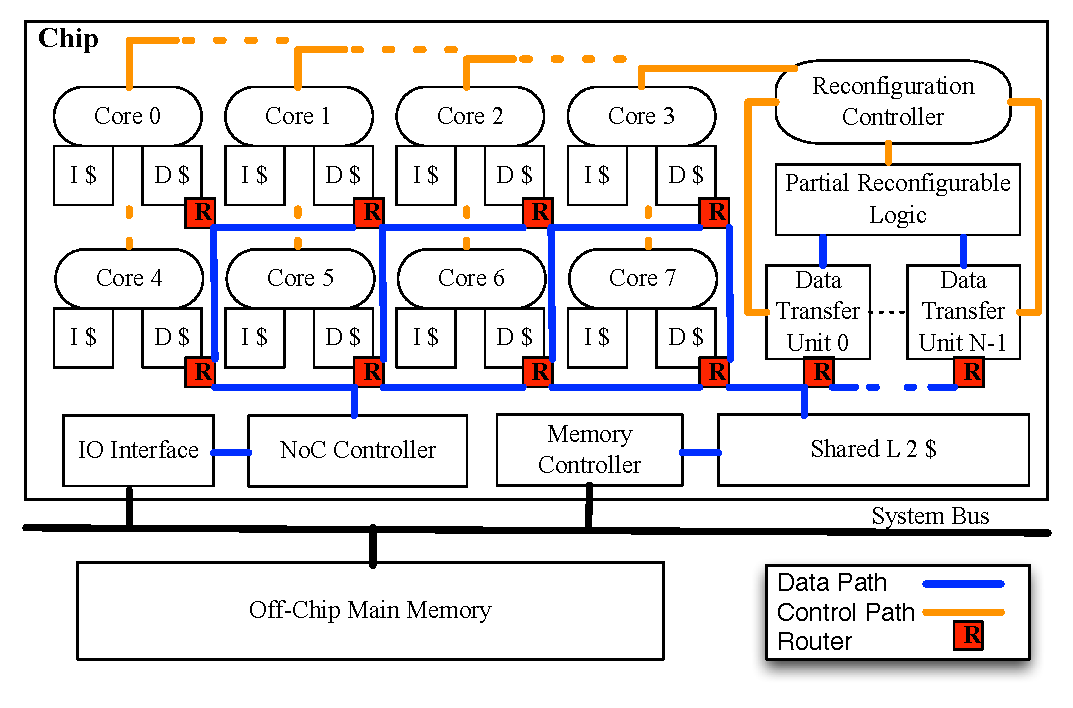
\includegraphics[width=4.0 in]{HPCA14-arch}
    \caption{Architecture Overview of {\em Transformer} }
    \label{fig_arch}
\vspace{-0.05in}
\end{figure}

Transformer's reconfigurable logic consists of computational resources
and {\em N} data transfer
units, supporting the instantiation of {\em N} independent accelerator
functions. The computational resources are organized in BRAM, DSP,
SLICEs as in a generic FPGA chip. The actual number of functions instantiated in the
programmable logic depends on the particular functions selected to
speed up at runtime and the resource requirements of the hardware
implementation of these functions. We study the architectural tradeoffs of 
reconfigurable logic and the number of cores in terms of performance
gains and power savings in Section \ref{sec_perf}.

Figure \ref{fig_reconfig_controller} depicts the three key components
in controlling the reconfiguration of accelerator logic:
reconfiguration controller, reconfigurable logic and data transfer
units. The reconfiguration controller is responsible for programming
new functions into the reconfigurable logic through new bit streams or
partial reconfiguration. Using control/status registers to record the
status of the reconfiguration logic, the controller receives
instructions from the middleware running on one of the cores, tracks
demands to various function calls, and makes decisions on what and
when to accelerate function(s).

The reconfigurable logic consists of a static region, a Partial
Reconfigurable Region (PRR) and an Internal Configuration Access Port
(ICAP). The static region contains necessary logics other than the
accelerator PRMs, such as clock module, interconnection interface and
memory control interface. The PRR can be divided into smaller
sub-regions and configured with different partial bit streams on
demand. ICAP is notified by the reconfiguration controller on what
kind of accelerator 
%PRMs ({\bf FIXME all different PRMs are located in
%  their fixed addresses}) 
should be configured and when to start. As a response, ICAP notifies
the controller about "resource full" and "(re)configuration done" by
writing to the specific bits of the control registers.

Each data transfer unit includes a pair of input and output buffers
that can be filled or drained by a DMA engine. The DMA engine is
responsible for bulk data transfer between the L2 cache and the
input/output buffers which are used as scratchpad memory for the
reconfigurable logic to complete necessary operations on the data. The
parameters such as memory addresses and data size of the DMA
operations are passed from the reconfiguration controller. TLB on each
of the data transfer unit is responsible for translating virtual
memory addresses to physical ones.


\begin{figure}
    \centering
    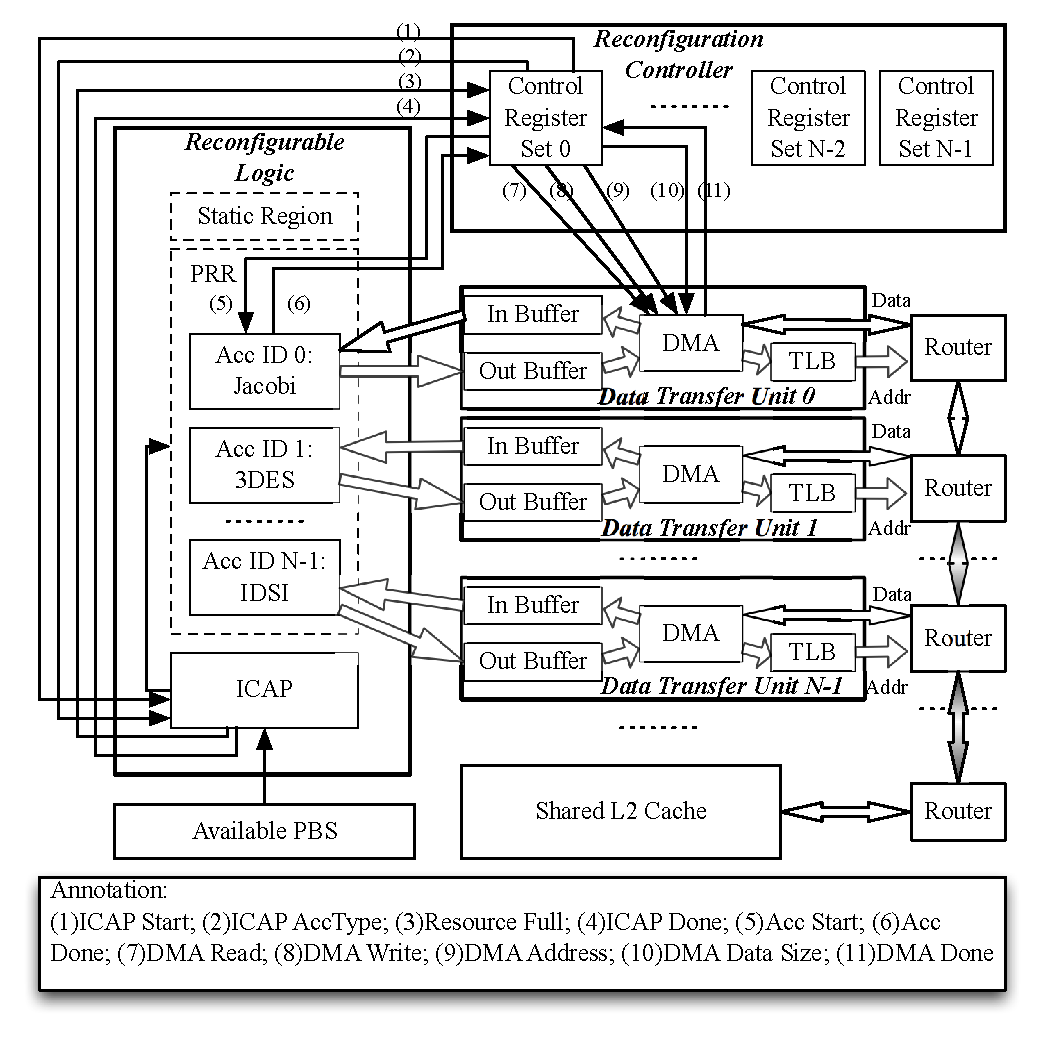
\includegraphics[width=4.0 in]{HPCA14-Controller}
    \caption{Transformer's Reconfigurable Logics and Controller}
    \label{fig_reconfig_controller}
\vspace{-0.05in}
\end{figure}


\subsection{Accelerator Invocation}

The invocation of accelerator from the software execution on a core is
done with specific accelerator instructions and control/status
registers. We illustrate how the accelerator is invoked in Figure
\ref{fig_Acc_Invoc}. We introduce {\em N} control register sets for
each to-be-instantiated accelerator and two new instructions to
invoke core-to-accelerator and accelerator-to-core execution path
transition. Each control register set contains three 32-bit registers:
general control register, DMA read register and DMA write
register. The general control register is responsible for ICAP control,
acceleration control and DMA control. The DMA read/write registers
contain read/write address of DMA operation source/destination
address. The specifications of the registers are described in Table
\ref{tbl_AccReg} and the two new instructions are listed as follows.

\begin{enumerate}
\item{\em readreg n}: read control register set with ID n and put the value into EAX register.
\item{\em writereg n}: write the value from EAX register into control register set with ID n.
%\item{\em accload AccReg n}: start configuring the type of accelerator
%  bitstream indicated by AccReg n into the reconfigurable logic. 
\end{enumerate}

\begin{table}[ht]
\scriptsize
\begin{center}
\begin{tabular}{|l|l|l|}
\hline 
\textbf{Register Name} & \textbf{Bits} & \textbf{Function}\\ 
\hline 
\hline
Gerneral Control &{\em Bit 0}   & ICAP start bit (IS)\\ 
\hline 
 &{\em Bit 1}   &  ICAP done bit (ID)\\ 
\hline 
 &{\em Bit 2-6} & ICAP accelerator type (IT 0-4)\\ 
\hline 
 &{\em Bit 7}   & acceleration start bit (AS)\\ 
\hline 
 &{\em Bit 8}   & acceleration done bit (AD)\\ 
\hline 
 &{\em Bit 9}   & DMA read enable (RE)\\ 
\hline 
 &{\em Bit 10}  & DMA write enable (WE)\\ 
\hline 
 &{\em Bit 11}  & DMA done (DD)\\
\hline
 &{\em Bit 12-15} & accelerator ID (ID 0-3)\\
\hline
 &{\em Bit 16-31} & DMA data block size (DS 0-15)\\
\hline
DMA Read Control &{\em Bit 0-31}  & DMA read address (RA 0-31)\\
\hline
DMA Write Control &{\em Bit 0-31} & DMA write address (WA 0-3)\\
\hline
\end{tabular} 
\caption{Control Registers for Reprogramming Accelerators.}
\label{tbl_AccReg}
\end{center}
\end{table}

The following is a brief introduction on how accelerator invocation
works. Note that all the set and reset operations are done by using
{\em readreg} and {\em writereg} instructions. These instructions are
encapsulated in customized wrapper functions, instead of being
directly used user applications.

\begin{enumerate}
\item If the reconfigurable controller decides to configure a specific
  combination of functions with the knowledge from middleware, the
  middleware will set the ICAP Start (IS) bit to start the
  reconfiguration process with the functions identified by ICAP
  accelerator type (IT 0-4) (This loading process will be skipped if
  the function is already configured in the accelerator logic.) At the
  same time, the middleware will prepare the data address and data
  block size by writing the DMA read address (RA 0-31) bits and DMA
  data block size (DS 0-15) bits.

\item Along with the reconfiguration process, we set the DMA Start
  (DS) bit to start reading the data from shared L2 cache or main
  memory into accelerator local input buffer until the buffer is full.

\item When the reconfiguration is done, ICAP will set the ICAP Done
  (ID) bit to enable the start of acceleration. By setting
  acceleration start (AS) bit, the Reconfiguration Controller causes a
  thread context switch on the corresponding core, which begins the
  execution of a different thread. The suspended thread will sleep
  until the acceleration done (AD) bit is set.

\item When the acceleration function is completed or the middleware
  decides to erase/change the accelerator function for the core,
  AccDone (AD) bit will be set and an interrupt will be generated to
  wake up the thread. Then the core will resume the previously
  sleeping thread, which will either continue a software path or get
  ready for the next accelerator invocation.
\end{enumerate}


\begin{figure}
    \centering
    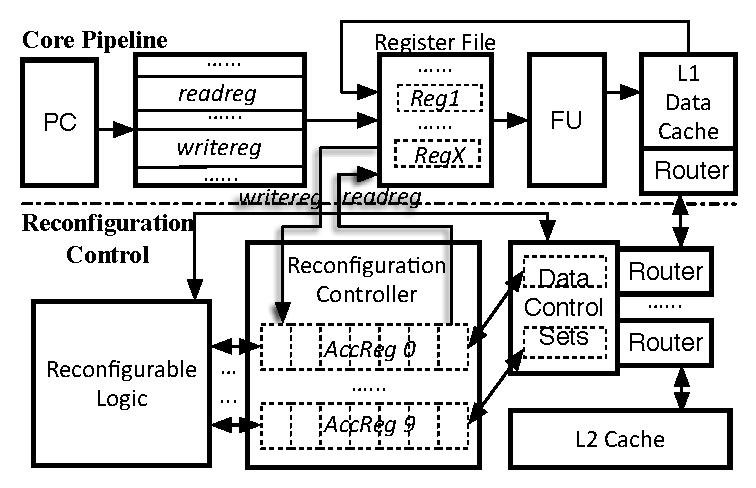
\includegraphics[width=4.0 in]{HPCA14-Acceleration_Invocation}
    \caption{Acceleration Invocation.}
    \label{fig_Acc_Invoc}
\end{figure}


To reduce the data transaction time from/to accelerators, a
combination of DMA and double buffering is used. 
Using double buffering, the accelerators can work on data residing in
their local memory while the DMA is fetching the next batch of data. A
TLB is located in between DMA and L2 cache to perform
virtual-to-physical address translation. This mechanism simplifies the
accelerator design, and guarantees the process isolation.


\section{Transparent Acceleration}
\label{sec_transacc}


Transparent acceleration of workloads is one of the design goals of
{\em Transformer}. Transparent acceleration refers to the speedup of
an application using hardware accelerators without the need of source
code access, recompilation or user intervention at run-time. We argue that such a feature is one of
the most important factors that enable the practical deployment of the
proposed heterogeneous architecture, because (1) the users'
workloads are typically present in the form of binary executables. Any
requirements on the access to source code and the capability of
rewriting the application impose tremendous obstacles for taking
advantage of a hardware accelerator; (2) the development environment
of user applications cannot be easily duplicated or emulated within
the run-time environment due to the complexity and variety of
compilers and libraries. As a result, the recompilation of an
application for hardware acceleration is either infeasible or
problematic; and (3) recompilation of user applications introduces
delays which are often unnecessary and/or intolerable. Therefore
transparent acceleration is critical for benefiting unpredictable
workloads with hardware accelerators.

To achieve transparent acceleration and ease the work of programmers,
we focus on the acceleration of commonly used libraries such as
libopenssl. Such libraries are made available with well known APIs to
their core functions, which are often the targets of acceleration. For
example, 3DES, a classic block cipher, is one of the many functions
within libopenssl, a suite of cryptography library implementing Secure
Sockets Layer (SSL) and Transport Layer Security
(TLS)\cite{wikissl} protocols. In the form of a dynamically linked
library, libopenssl provides entry points to its functions like
3DES. We propose to add a layer of wrapper functions that profiles and
intercepts the calls from user applications to the libraries that can
be accelerated with programmable logic. 


\begin{figure}
    \centering
    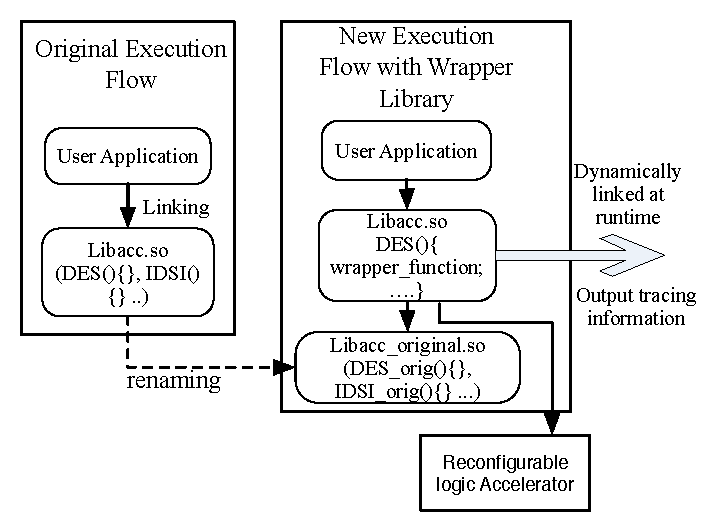
\includegraphics[width=4.0 in]{HPCA14-wrapperlib}
    \caption{Original and Modified Execution Flow}
    \label{fig_transacc_flow}
\end{figure}

Wrapper functions are presented in the form of dynamically linked
libraries, replacing the original libraries by renaming. As a result,
the calls to the original dynamic library are directed to wrapper
functions due to the linker stub \cite{linkerstub}. The modified
execution flow is shown in Figure \ref{fig_transacc_flow}.  The
original dynamic linked library is renamed by adding suffix
{\em ``\_original''}, so are its functions by rewriting its symbol table. We
create our new dynamic-linked library with the same name as the original library, and
incorporate a wrapper function to intercept all the library calls
(call to the original function names) and
redirect them to either the original software library or the hardware accelerator.

The responsibilities of wrapper functions are two folds: (1) {\em profiling}:
a wrapper library record the number of calls to each of the
library functions. Such counters reflect the demands to individual
functions (e.g. 3DES), which are used by the reconfiguration
controller to determine which functions are to be accelerated in
programmable hardware. We provide details of the algorithms for such
run-time reconfiguration in Section \ref{sec_runtime_reconfig}; and (2)
{\em function call redirection}: a wrapper function directs the
execution flow to an appropriate path, i.e. either continuing software instruction execution on a core or
acceleration with a programmable hardware unit. The wrapper functions
are aware of the currently accelerated functions on the programmable
accelerators, and such knowledge is updated by the reconfiguration
controller. If the required function is currently supported in the hardware
accelerator, this call and subsequent ones to the particular library
function(s) are redirected to the accelerator, thus reducing execution
time.

The library based transparent acceleration benefits the dynamically
linked applications which are well supported in modern operating
systems such as Windows and Linux. For statically linked applications,
although the dynamic library based transparent acceleration is limited
in detecting library calls and redirecting instruction flow to
hardware accelerators, we argue that such limitation is not inherent
to the proposed heterogeneous architecture. A user can still
incorporate our wrapper functions into the application so that the
calls to compute-intensive functions are instrumented, and the
subsequent calls are redirected to programmable accelerators when the
run-time system determines that the particular function should be sped
up with a hardware based accelerator at the current moment.
We show a sample acceleration function call process in Algorithm \ref{alg_sample_func}.

\begin{algorithm}[htb]
\scriptsize
\caption{Sample Acceleration Function Call}
\label{alg_sample_func}
\begin{algorithmic}[1]
\STATE {\em In User Function:}
\STATE {Call: DES (arg1, arg2, arg3) \newline}
\STATE {\em In Wrapper Function DES(arg1, arg2, arg3):}

\IF {DES is called}
	\STATE {RequestCounter ++ \COMMENT{Increase Request Counter by 1}}
	\IF {Request tracking time window is finished}
		\STATE{$D_{x} = \sum_{i=1}^{H}C(x,i)$ \COMMENT{Total demand}}
		\STATE{$DC_{x} = \sum_{i=1}^{H-1}(|C(x, i+1)-C(x, i)|)$\COMMENT{Demand changes}}
		\IF {Use naive scheduling}
			\STATE{$P_x = a \times D_x + (1-a) \times DC_x$ \COMMENT{Priority of this function}}
		\ENDIF
		\IF {Use Bandwidth/Speedup First scheduling}
			\STATE{$P_x = $ the result of 2D-knapsack combination}
		\ENDIF
	\ENDIF
	\IF {Function DES meets the requirement of being scheduled}
		\STATE{$ConfigStart \leftarrow 1$; $AccType \leftarrow 0$ \COMMENT{3DES is type 0}}
		\STATE {$ArgNum \leftarrow 3$; $AccPtr \leftarrow \& arg1$; $DS \leftarrow 1$}
		\IF {$ConfigDone = 1\quad\AND\quad DD = 1$}
			\STATE{$AccStart \leftarrow 1$}
		\ENDIF
		\IF {$AccDone = 1$}
			\STATE{Get back to previous thread.}
		\ENDIF
	\ELSE
		\RETURN $DES(arg1, arg2, arg3) \COMMENT{\text{Software  Version}}$
	\ENDIF
\ENDIF

\end{algorithmic}

\end{algorithm}










\section{Run-time Reconfiguration }
\label{sec_runtime_reconfig}

\subsection{Overview}
\label{subsec_runtime_reconfig_overview}

Run-time reconfiguration refers to the decisions made by the controller
to accelerate certain software libraries, 
as determined by the run-time workload characteristics, as well as how to effectively assess the
workloads periodically. The heart of reprogramming hardware
accelerators at run-time lies in the algorithms as well as the mechanisms employed to
identify software functions that should be accelerated, keeping in mind the goals of sharing
the memory and logic resources as well as maximizing the resource utilization of the
reconfigurable logic. Since reprogramming the accelerator logic 
introduces a delay, we do not want the aforementioned overhead to outweigh the benefits of accelerating time-consuming
tasks. We propose a reconfiguration controller which addresses three
questions.
First, what it the most effective way to track the demands of the candidate workloads? 
Second, when should the acceleration logic be reprogrammed?
Third, which accelerator or combination of accelerators should be instantiated?


The aforementioned questions are answered in two steps:
demand tracking and request scheduling. As described in
Section \ref{sec_transacc}, the first step is to intercept all of the
library calls with wrapper functions and keep track of the demands
using a table of counters called Request Counters (RC). The RCs
are regarded as a request log that contains updated information for the most
recent time window. In the second step, heuristic algorithms are applied in order to
schedule the requested function within the hardware accelerators. 
The corresponding algorithms are described in Section \ref{subsec_combo}. 

\subsection{Demand Tracking} 

The demands of computing a candidate function are tracked by the
wrapper function library. The library maintains a table of candidate
hardware accelerators along with the corresponding functions they are designed to speed up. Each call
to a function is intercepted and recorded by the wrapper function, which is then used as an
index into the table in order to increment the corresponding request counter. The
counters serve as input metrics to the scheduling algorithm, which determines the appropriate
functions to accelerate. Tracking the demands only requires performing two memory operations, a table
lookup, a read, followed by a table update, a write.
The overhead of maintaining the counters is trivial, even when the number
of accelerators scales into the hundreds. Specifically, each counter
update is only performed once for each library function call.  By comparison, the library function itself is typically time-consuming, in the order millions of cycles. Moreover, the counters are reset periodically in order to record the most recent demands. 


In the presence of dynamic workloads and heterogeneous processing
elements, which include general-purpose cores as well as programmable accelerators, there
could be multiple, time-dependent candidate functions to accelerate.
 The acceleration of the workload turns into an optimization
problem where the objective is to schedule tasks on multiple
processors in order to minimize the execution time. Given that Hochbaum et
al. have proven similar scheduling on uniform processors is NP-hard
\cite{hochbaum88}, the scheduling on heterogeneous processing 
elements must also be NP-hard. Therefore, we derive heuristics to address
the remaining two questions.
 Specifically, we address the second question with
the heuristics for determining the reconfiguration timing in
Section \ref{subsec_ranking}, and the third question with the heuristics for
scheduling and combining accelerators in Section \ref{subsec_combo}.

\subsection{Request Ranking}
\label{subsec_ranking}

Each time function acceleration requests are detected by the
wrapper library, we increment the corresponding request counter in a
time window of length $T$ before resetting it in the next window. 
Not only are we interested in the number of calls within a time window $T$, but also the {\em changes} in the demands
between subsequent time windows. Specifically, the dynamic workloads
could experience demand fluctuation, implying that the historical trend in the
past time windows is just as important as the number of calls in one or
more time windows.
Smaller values for $T$ lead to frequent counter resets and trace the trend
of demands with finer granularity, while larger values for $T$ avoid
oversampling the demands as well as unnecessarily frequent reprogramming of the accelerators. Therefore, the value of $T$ should be chosen
appropriately such that it does not add significant overhead when
comparing the execution times of the applications under study, while being sufficient
to capture the details of the changes in demand for the acceleration requests. 

We maintain an array of counters $C(x, i)$ collected in the past $R$
time windows, where $x$ represents the corresponding accelerator
function and $1<i<R$. At run time, there exists an $f \times R$
matrix $M$ that reflects the demands for $f$ accelerator functions in
the past $R$ time windows.  After obtaining $M$, we use the following
two metrics to evaluate the total demand $D_x$ and the rate of demand
changes $DC_x$ for every function $x$: $D_{x} = \sum_{i=1}^{H}C(x,i)$
and $DC_{x} = \sum_{i=1}^{H-1}(|C(x, i+1)-C(x, i)|)$.  The priority
$P_x$ of function $x$ is then calculated as $P_x = a \times D_x +
(1-a) \times DC_x$. We set $a$ to be 0.5 in our implementation given that we
regard the changes in demand to be as important as the total number of demands. $P_x$
is used to rank the accelerators requests in descending
order. Changes that occur in the ranking from the past time window trigger
reprogramming the accelerator functions in the on-chip logic. We regard the aforementioned scheduling strategy as the baseline and denote it as ``na\"{\i}ve'' in the performance evaluation.

\subsection{Combining Accelerators}
\label{subsec_combo}



Combining acceleration functions to maximize the utilization of reconfigurable logic
allows more effective speedup and power savings.

As each accelerator function consumes a certain amount of
on-chip resources such as LUT, memory, and data access
bandwidth to achieve a particular speedup factor, as shown in Table
\ref{tbl_benchmark}, the choice of accelerators to maximize gains
under resource constraint is a combinatorial optimization problem, i.e., knapsack problem. We will discuss two variants of knapsack problem
applicable in our accelerator scheduling algorithm: one is 0-1
knapsack problem, i.e., an acceleration function is either chosen or not
chosen;  the other is bounded knapsack problem: up to $n$ copies of
the same acceleration function can be instantiated as independent
engines into the accelerator. With the total resource available to the programmable accelerator as
a constraint, we consider two different prioritization strategies to minimize the
execution time: memory bandwidth utilization first and acceleration
speedup first when solving the knapsack problems.

\subsubsection{Mathematical Model}

We model an accelerator function as $A(SLICE, DSP, BRAM, Bandwidth, Speedup)$,
where {\em SLICE, DSP, BRAM} are logic, application-specific blocks and
memory cells resources, respectively, consumed by the function when it is
instantiated in the reconfigurable logic unit. {\em Bandwidth} is the
requirement of the function on data bus in order to keep the unit
busy. {\em Speedup} is the effective speedup of an accelerated function on the
reconfigurable logic compared to its software implementation. 

\begin{table*}[ht]
\scriptsize
\centering
\begin{center}
\begin{tabular}{|c|c|c|c|c|c|c|c|c|c|c|c|}
\hline 
\textbf{Accelerators}& \textbf{SLICE} & \textbf{SLICE \%} & \textbf{FF} & \textbf{FF \%} & \textbf{LUT} & \textbf{LUT \%} & \textbf{BRAM} & \textbf{BRAM \%} & \textbf{Bandwidth MB/s} & \textbf{Speedup} & \textbf{Power W} \\ 
\hline
\hline  
3DES          & 1148  & 24.7  & 807  & 8.7  & 1081 & 11.6  & 8    & 40   & 392   & 25.2     & 0.157\\ 
\hline 
IDSI          & 1637  & 35.2  & 530  & 5.7  & 891  & 9.6   & 0    & 0    & 970   & 13.1     & 0.235\\ 
\hline 
SLAM-C        & 812   & 17.4  & 973  & 10.4 & 854  & 9.2   & 0    & 0    & 479   & 33.0     & 0.156\\ 
\hline 
SLAM-J        & 983   & 21.1  & 1027 & 11.1 & 872  & 9.4   & 0    & 0    & 458   & 29.0     & 0.147\\ 
\hline 
SURF          & 1877  & 40.3  & 1163 & 12.5 & 705  & 7.6   & 5    & 25   & 983   & 25.0     & 0.161\\ 
\hline 
Segmentation  & 2918  & 62.7  & 930  & 10.0 & 630  & 6.8   & 12   & 60   & 848   & 45.5     & 0.178\\ 
\hline 
SmithWaterman & 626   & 13.4  & 1285 & 13.8 & 1034 & 11.1  & 20   & 100  & 403   & 36.6     & 0.182\\ 
\hline 
Jacobi        & 1201  & 25.8  & 1431 & 15.4 & 1218 & 13.1  & 2    & 10   & 1112  & 30.6     & 0.153\\ 
\hline 

\end{tabular} 
\caption{Benchmark accelerator logic cost, bandwidth, speedup and
  power {\em (Use Xilinx SPARTAN 3E as a reference)}} 
\label{tbl_benchmark}
\end{center}
\end{table*}

Table \ref{tbl_benchmark} summarizes the library functions under
study. These functions (explained in detail in \cite{accstore}) are
representative time-consuming workloads in a wide range of application
domains.  In this table, all data (except bandwidth consumption and
speedup) are derived from the open source synthesizable accelerator
store \cite{accstore}. We measure their memory bandwidth with Intel
VTune Amplifier XE \cite{vtune}. The speedup of each accelerator is
calculated by dividing execution time of one iteration of the software
benchmark on a 1.6 GHz single core by its corresponding hardware design
on a 200 MHz FPGA. {\em Transformer} applies Xilinx Spartan-3E XC3S500E
FPGA \cite{spartan3e} as a reference on-chip accelerator, which has a
comparable number of transistors ({$100\sim300$ million (500K gates)})
as eight Atom 330 cores ({$\sim 47$ million per core})
\cite{atom-spec}. The total number of SLICE on chip is 4656, LUT is
9312, FF is 9312, DSP48 is 768 and BRAM is 20. We also show the
percentage of resource consumption of each acceleration function. It
can be observed that the numbers of SLICEs and BRAMs are two major
resource constraints. Therefore, we reduce the multi-dimensional
knapsack problem to a two-dimension problem. That is, we consider the
percentage of SLICEs and BRAMs of each benchmark as the two weights in
the knapsack model. The memory bandwidth utilization and speedup are
regarded as two objective functions for reducing the total execution
time of memory-bound and compute-bound applications, respectively.

In the memory bandwidth-first combination, we attempt to maximize the
total bandwidth $\sum_{i=0}^{n}(BW_i \times Acc_i) $ subject to
$\sum_{i=0}^{n}(w_i \times Acc_i) $, where $Acc_i$ $i \in {1,2,3,
  ... ,n}$ denotes different accelerator functions, $BW_i$ being the
bandwidth cost and $w_i$ being their weight, i.e. the SLICE resource
demand. In the speedup-first combination selection, we focus our
efforts on maximize the speedup metrics $\sum_{i=0}^{n}(SP_i) $, where
$SP_i , i \in {1,2,3, \ldots, n}$ denotes the speedup of each
accelerator. We attempt to maximize the two metrics because improving
the system bandwidth utilization and choosing a function with
significant speedup are two main approaches to improve the system
performance. For example, our experiment results shows that if we
offload memory-bound benchmarks such as IDSI, SURF, Segmentation and
Jacobi to reconfigurable logics with higher memory bandwidth, we can
expect better overall performance and power efficiency. These
heuristics are shown to be effective through extensive experiments
described in Section \ref{sec_perf}.

\subsubsection{Dynamic Programming}

Both two-constraint 0-1 knapsack problem and two-constraint bounded knapsack problem can be solved
by dynamic programming. 

\noindent{\em 0-1 Knapsack Problem Solution}

Assume we have $n$ acceleration functions to choose from, which are
annotated as $Acc_1$, $Acc_2$, \ldots, $Acc_n$. All $n$ items have
their two-constraint weight $a_i$, $b_i$ and value $v_i$, $i \in [1,
  2, \ldots, n]$. Then we define $V[i, a, b]$ to be the current
maximum value we can obtain with a weight less than or equal to $a$
and $b$ using first $i$ accelerators. The upper limit of two weights
are $A$ and $B$. We derive recursive equations for $V[i, a, b]$:

\begin{equation}
V[i, a, b] = V[i-1, a, b] \quad \text{if} \quad a_i > a, b_i > b,
\end{equation}
meaning if adding a new accelerator exceeds the current
two-dimensional weight limit, then we shall not choose the new
accelerator and the total value will not change, and
\begin{equation}
\begin{array}{c}
	V[i, a, b] = max(V[i-1, a, b], V[i-1, a - a_i, b - b_i] + V[i, a, b])\\
	\text{if} \quad a_i \leq a \quad b_i \leq b.
\end{array}
\end{equation}

Algorithm \ref{alg:0-1-knapsack} describes how we solve two-constraint 0-1
knapsack problem to select a set of accelerator functions. 

\begin{algorithm}[htb]
\scriptsize
\caption{ 0-1 Knapsack Problem Solution}
\label{alg:0-1-knapsack}
\begin{algorithmic}[1] 
\FOR {each $a \in [0, A]$}
	\FOR {each $b \in [0, B]$}
    	\STATE $ V[a, b] = 0; $
    \ENDFOR
\ENDFOR
\FOR {each $i \in [1, n]$ } 
    \FOR {each $a \in [A, a_i]$ }
    	\FOR {each $b \in [B, b_i]$}
    	
        	\IF {$j \geq w[i]$}
            	\STATE $V[i, a, b] = max(V[i-1, a, b], V[i-1, a - a_i, b - b_i] + v[i, a, b]) $
        	\ELSE
            	\STATE $V[i, a, b] = V[i-1, a, b]$
        	\ENDIF
        \ENDFOR
    \ENDFOR
\ENDFOR
\end{algorithmic}
\end{algorithm}

\noindent{\em Bounded Knapsack Problem}

The two-constraint bounded knapsack problem can be solved in a similar
way as 0-1 knapsack problem. Using two extra annotations, $C$ as the
maximum number of acceleration function we can request for a certain
function, and $k_i$ as the number of functions $i$ we choose, we can
derive a similar recursive equation for $V[i, w]$.

\begin{equation}
V[i, a, b] = V[i-1, a, b] \quad \text{if} \quad a_i > a, b_i > b
\end{equation}

and

\begin{equation}
	\begin{array}{c}
		V[i, a, b] = max(V[i-1, a, b], V[i-1, a - k_i\times a_i, b - k_i\times b_i] \\
		+ k_i\times V[i, a, b])\\
		\text{if} \quad a_i \leq a \quad b_i \leq b
	\end{array}
\end{equation}

The algorithm for bounded knapsack problem is similar to Algorithm
\ref{alg:0-1-knapsack}, thus not elaborated due to space limit.





\begin{flushright}

\end{flushright}\section{Performance Evaluation}
\label{sec_perf}
 

\subsection{Simulator Overview}
To evaluate the performance and power consumption of the proposed
architecture, we simulate the multi-core heterogeneous architecture
by extending Multi2Sim - a superscalar, multithreaded and multicore
simulator - with a reconfigurable accelerator unit. 
 The specification of our simulated architecture is shown in Table
\ref{tbl_parameters}. The processor core technology and operating
frequency is modeled based on the Atom 330 processor, and we set the
number of cores as eight in the baseline configuration. Later we vary the
number of cores to explore the area allocation to accelerators and cores. 
The ICAP interface runs at 100 MHz although over-clocking ICAP is
possible in practice\cite{Hansen:2011dt}.

\begin{table}
\scriptsize
\begin{center}
  \begin{tabular} { | l | l | }
    \hline
    \textbf{Item} & \textbf{Parameter} \\
    \hline
    \hline
	Core & 8 \\
	\hline
	Core Spec & 45nm @ 1.6 GHz \\
	\hline
	Accelerator Spec& 45nm @ 200 MHz \\
	\hline
	ICAP & 32 bit bus width @ 100 MHz \\
	\hline
	L1 Instr/Data \$ Size (KB) & 32 \\
	\hline
    L1 Instr/Data \$ Associativity & 4\\
    \hline
    L1 Instr/Data \$ Block Size (Bits) & 64\\
    \hline
    L1 Instr/Data \$ Number of Sets & 128\\
    \hline
    L1 Instr/Data \$ Latency (Cycles) & 3 \\
   	\hline
   	L2 Cache Size (MB) & 4 (shared) \\
   	\hline
    L2 Associativity & 8\\
    \hline
    L2 Block Size (Bits) & 512\\
    \hline
    L2 Number of Sets & 1024 \\
    \hline
    L2 Latency (Cycles) & 20\\
    \hline
    CPU Cache Coherence & MOESI\\
    \hline
    Accelerator Data Buffer Size (KB) & 8 \\
    \hline
    Accelerator Data Buffer Coherence & MOESI\\
    \hline
    Memory Size (GB) & 8 \\
    \hline
    Memory Latency (Cycles) & 200 \\
    \hline
    Memory Data Block Size (Bytes) & 512\\
    \hline
    Memory Page Size (Bytes) & 8192\\
    \hline
    Memory Replacement Policy & Pseudo LRU\\
    \hline
    Network Topology & 2-D Mesh\\
    \hline
    Network Bandwidth (MB/s) & 1024\\
    \hline
  \end{tabular}
\caption{Hardware Specification.}
\label{tbl_parameters}
\end{center}
\end{table}


To model the profiling and scheduling overheads in the simulations,
we evaluate the overhead of the profiler within the wrapper function and the
three scheduling methods - na\"{\i}ve, bandwidth first or speedup first. For
the worse case, the profiler and wrapper function overheads take up
to 0.017 \% per profiling window time and the worse case happens only
when the reconfiguration controller accepts the current acceleration
request within the profiling window. The two knapsack combination
scheduling algorithms introduce more overhead than na\"{\i}ve scheduling. However, further evaluation shows that the overhead of both bandwidth
first and speedup first algorithms introduce an neglectable overhead of 0.130 \% per profiling window. 

\subsection{Benchmarks}
We use all the eight acceleration functions from the
open-source accelerator store \cite{accstore} to build a synthetic
workload that simulates dynamic workloads in cloud and mobile
environments (we defer using real-world cloud applications to our
future work).  These applications cover a wide range of areas
including encryption/decryption ({\em 3DES} \cite{openssl}), numerical
calculation ({\em Jacobi} \cite{jacobi-wiki}), vision and navigation
({\em SLAM-C and SLAM-J} \cite{openslam}), feature detection (SURF and
IDSI \cite{opencv}), image processing ({\em Segmentation}
\cite{segmentation-wiki}) and bioinformatics ({\em Smith-Waterman}
\cite{smithwaterman-wiki}). Besides, these software applications have
corresponding accelerator implementation which provide
performance/area details. Minor modifications are done to generate the
final benchmark mixture, including preparing the input data set for
each function and creating multiple threads.

To emulate the dynamics of workload arrival, we model the inter-arrival time between
each benchmark as Poisson distribution. The average
inter-arrival time is set as 500,000,000 (312.5 ms
in real time if system is running at 1.6 GHz), which is close to the
cycle time of one iteration of our shortest benchmark IDSI. We compare
this Poisson arrival pattern with default pattern - continuous
arrival, i.e. inter-arrival time is zero.

\subsection{Modeling Accelerators}
As there is no accelerator modeled in the stock Multi2Sim simulator,
so we modify a general purpose core to simulate a reconfigurable
accelerator unit. We make our best effort to model the
computation, memory access and reconfiguration delays  based
upon prior work and our own studies on the benchmarks. 

We model the timing of each accelerator by using their different
speedup values reported in the prior work as listed in Table
\ref{tbl_benchmark}. The speedup numbers are scaled to the 
operating frequencies of cores and reconfigurable logic used in our
simulations. 

We are interested in understanding the memory access
patterns (e.g. footprint, data size and frequency) and modeling
them in accelerators with high fidelity in the simulations. Towards this goal, we profile the memory
activities by logging memory access traces for each 
acceleration function.
Figure \ref{fig_mem_access} illustrates the memory access pattern of
two benchmark applications: Jacobi and SLAM-J. The horizontal axis is
the time of the access, and the vertical axis is the address within a
page range. In this way, we observe the temporal and spatial
characteristics of the memory accesses. It can be seen that {\em
  Jacobi} has a much larger number of  accesses than SLAM-J, and the
accesses span over a wider address range. We model such the memory
access patterns when simulating accelerators, besides visually
differentiating memory bound applications from the computation intensive
ones. 

The overhead of a DMA transfer is modeled with the approximation
formula from \cite{Saidi:2012}: $ T(s) = I + \alpha \times b \times
s$, where $I$ is the fixed initial cost which includes command issuing
and TLB translation, $\alpha$ is the transfer cost rate in
$cycle/byte$, $b$ is the basic block size and $s$ is the super block
size. Since DMA command and TLB translation are already modeled in wrapper libraries and the
stock Multi2Sim simulator separately, $I$ is 0 in this case. We choose $\alpha$
as 2 cycles/byte as an average number \cite{Saidi:2012}. $b$ and $s$
are determined by specific functions.


\begin{figure}
    \centering
    \includegraphics[width=6.0in]{Mem-Access}
	\caption{Memory access pattern of Jacobi (left) and SLAM-J (right)}
\label{fig_mem_access}
\end{figure}


The input/output buffers on each of the accelerators are modeled by
modifying the Multi2Sim cache models. The MOESI cache coherence
protocol remains effective. TLBs are employed to handle virtual memory
address translation.  We have studied the impact of the input/output
buffers size on the performance of {\em Transformer}'s reconfigurable
logics. The results (not depicted here) reveal that the performance of
accelerator increases significantly from 8KB to 32KB, beyond which no
substantial improvement is observed. So our simulations use 32KB as
the default buffer size.

The partial reconfiguration delay $T_R$ is modeled as $ T_R = \frac{S_{pbs}}{ B_{ICAP} / C_{ICAP}} $,
where $S_{pbs}$ is the size of
partial bitstream, and $B_{ICAP}$ and $C_{ICAP}$ are the bus bandwidth
and cycle time of ICAP.
Since partial reconfiguration time depends on the size of partial bit
stream, we conservatively model the reconfiguration time with the
largest bitstream size among all the benchmarks in our simulations. 


\subsection{Power Model}
The general purpose cores' dynamic and static power consumption are
estimated by using HP McPat v0.8 \cite{mcpat}. The power consumption of reconfigurable logic
is modeled as follows. We keep track of the numbers of
each logic elements (SLICE, FF, DSP48, BRAM, etc.) used by the
accelerator functions at run time, and use them as input data to Xilinx Power Estimator
\cite{xpe} for calculating reconfigurable logic's power consumption.  
We scale the power of the reconfigurable logic to the 45 nm technology
so that both cores and accelerators are at the same technology
scale. The total power consumption is the sum of the power of
reconfigurable logic  and  the power number reported by McPat for the
cores. 


\subsection{Simulation Results}
\label{sec_simu_result}

\subsubsection{Speedup of Multiple Copies of a Single Workload}

We first study the effectiveness of {\em Transformer} on single function 
workloads. A software thread repeatedly executes a single function
(e.g. 3DES) and then we gradually increase the number of threads. In this setting, both 
scheduling methods will select the same accelerator since the wrapper function
intercepts only one kind of library calls. As a result, we only compare the architectures with
or without accelerators. 
Figure \ref{fig_num_of_apps} shows that the performance speedup on the y
axis while the x axis shows the increasing number of threads. The
baseline performance is the execution time of $k$ threads on multicore
architecture without the accelerator. We can
observe that the speedup for 3DES is significant ($\sim$14x) when the number of threads is
within two, beyond which the speedup reduces. This is because the
resources available in the accelerator logic only allow up to two
3DES accelerator functions instantiated. The remainder of the threads
end up being executed as software on the cores, so the speedup is not
as significant as earlier cases.  Other functions
experience similar trends but the number of acceleration function
copies differs from benchmark to benchmark.   

The disparity in reconfigurable resource requirements among benchmarks
validates the opportunities for combining accelerators. Further
analysis shows that 3DES accelerator function requires 40\% of 
the BRAM resources of the reconfigurable logics, so only two copies of
3DES functions can be instantiated. However, other types of
resources such as LUT remain abundant for accommodating
functions such as SLAM-C, which requires only 9.2\% of the LUTs and no
BRAMs. We later illustrate the run-time accelerator instantiation and combination in Figure
\ref{fig_acc_timeline}.   

\begin{figure}
    \centering
    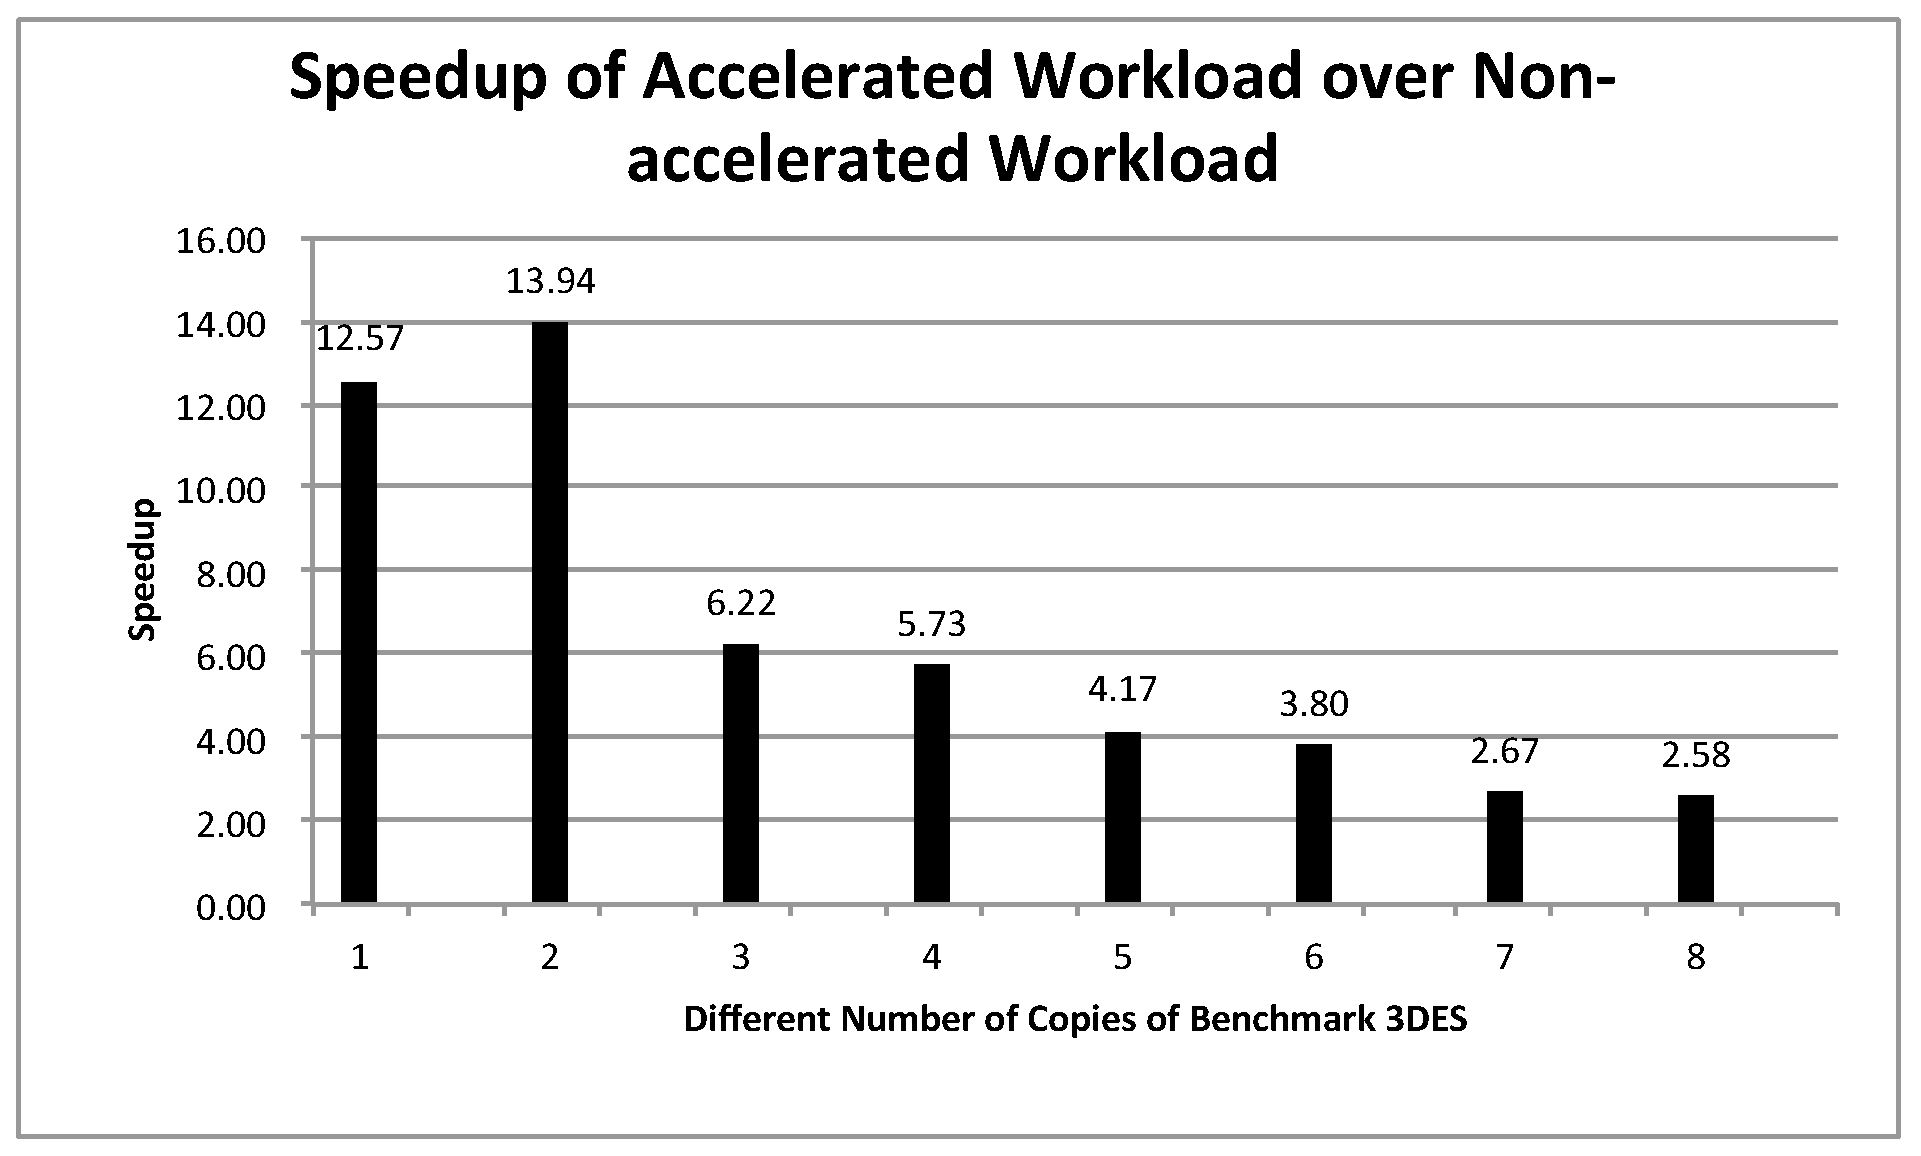
\includegraphics[width=4.5in]{Increase-Num-of-Apps}
    \caption{Speedup of Multiple Copies of a Single Workload Type}
    \label{fig_num_of_apps}
\end{figure}

\subsubsection{Speedup and Energy Efficiency of Workload Mixtures}

With a mixture of the workloads, the instantiation of accelerator
functions is subject to the run-time demands and the logic resource
constraints. We execute the synthetic workloads on {\em Transformer} with eight
cores and one reconfigurable logic unit of the size of an Xilinx
Spartan 3E. The workload's arrival follows either a Poisson process or
a back-to-back fashion. We issue 100 thousand billion instructions of
the benchmark bundle and record the number of completed functions and
cycle times. 

\begin{figure}
    \centering
    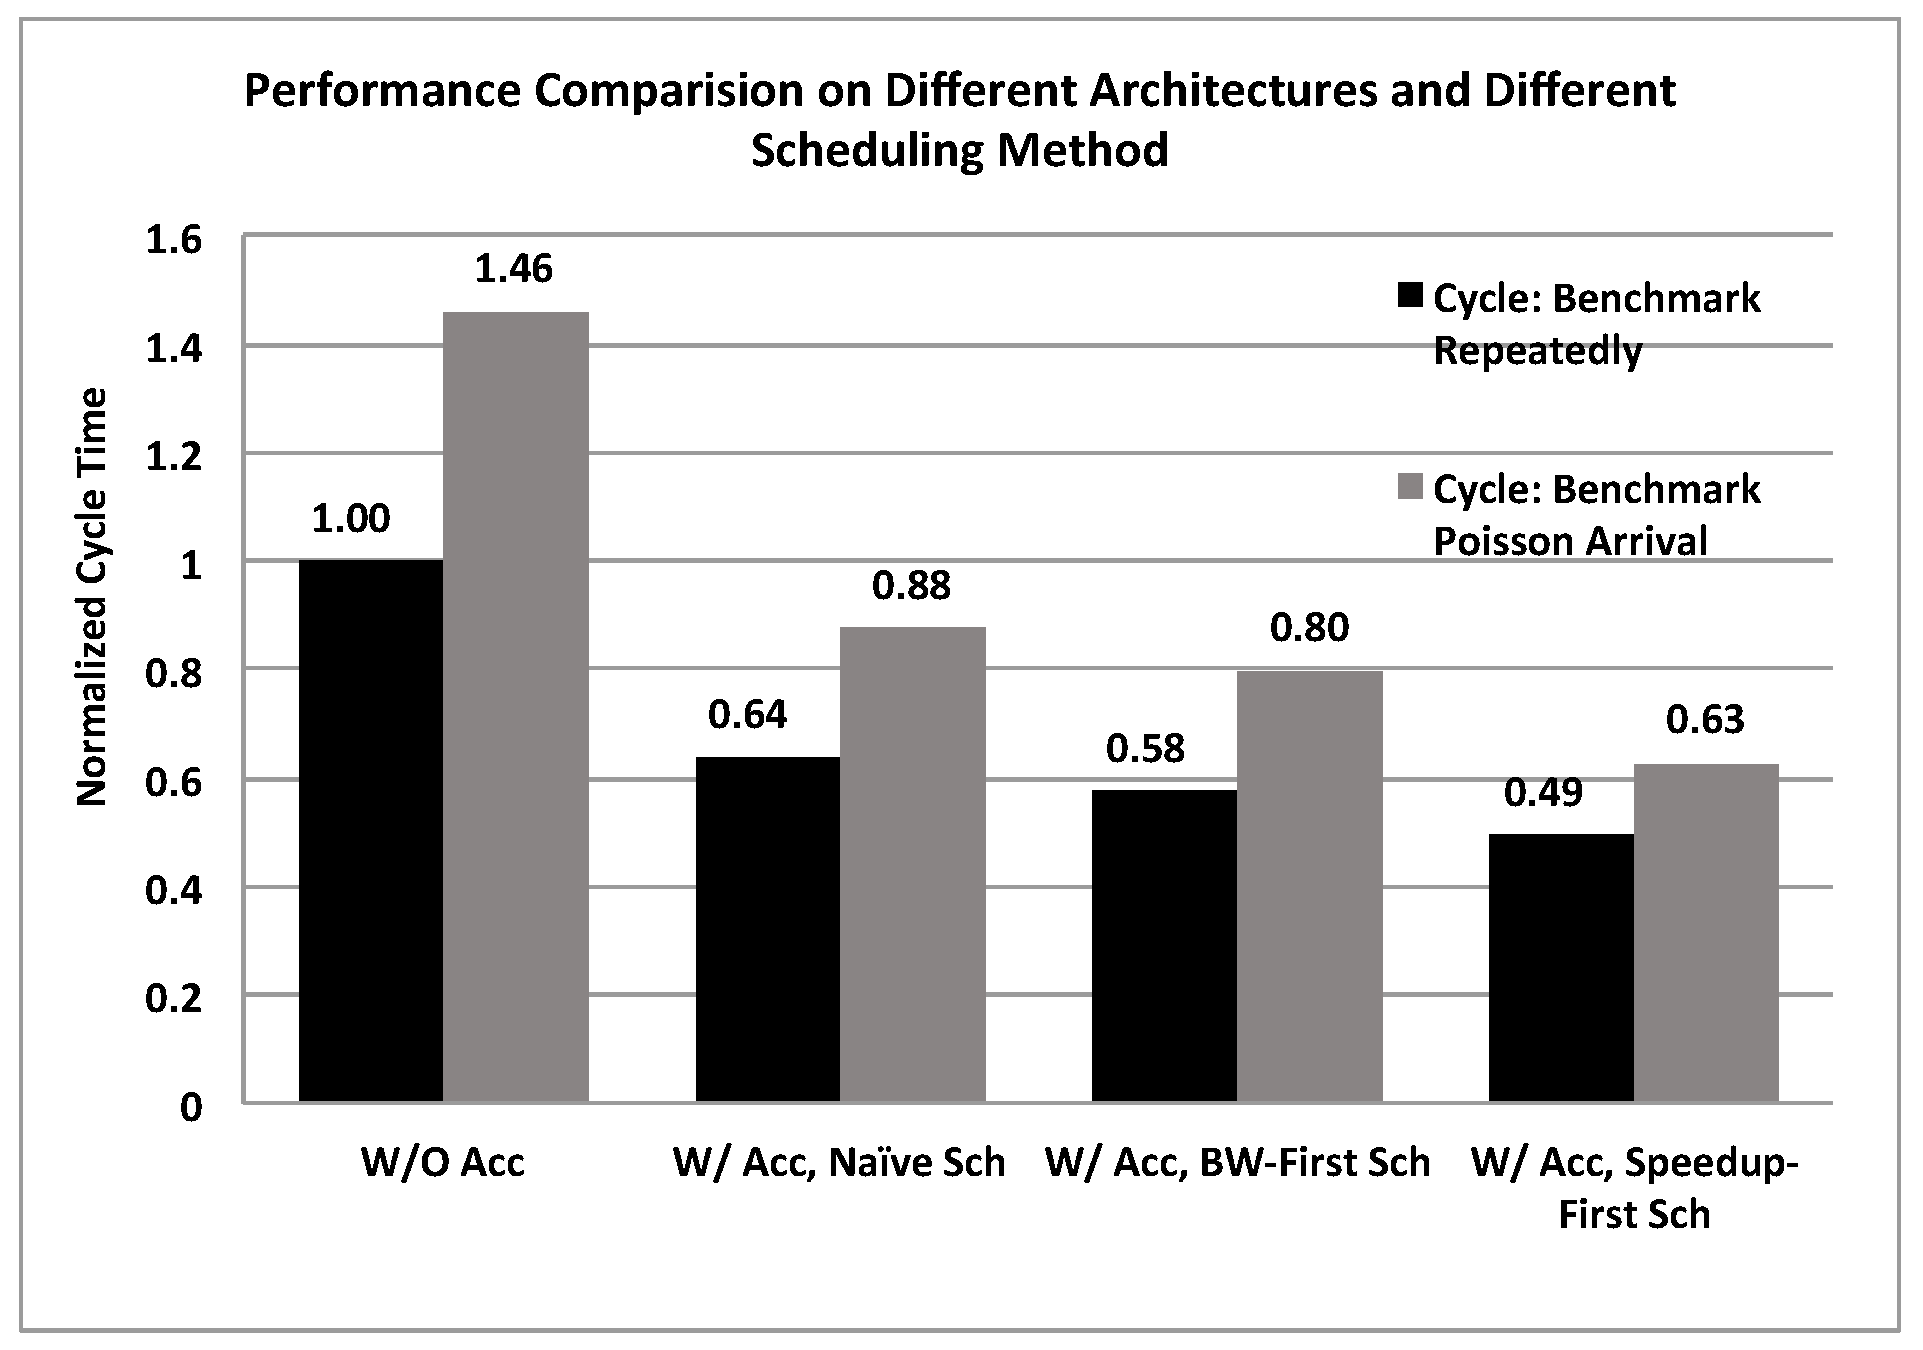
\includegraphics[width=4.5in]{Cycle-8core}
    \caption{Performance Comparison of Accelerated Architecture and Scheduling Algorithms.}
    \label{fig_8core_cycle}
\end{figure}

\begin{figure}
    \centering
    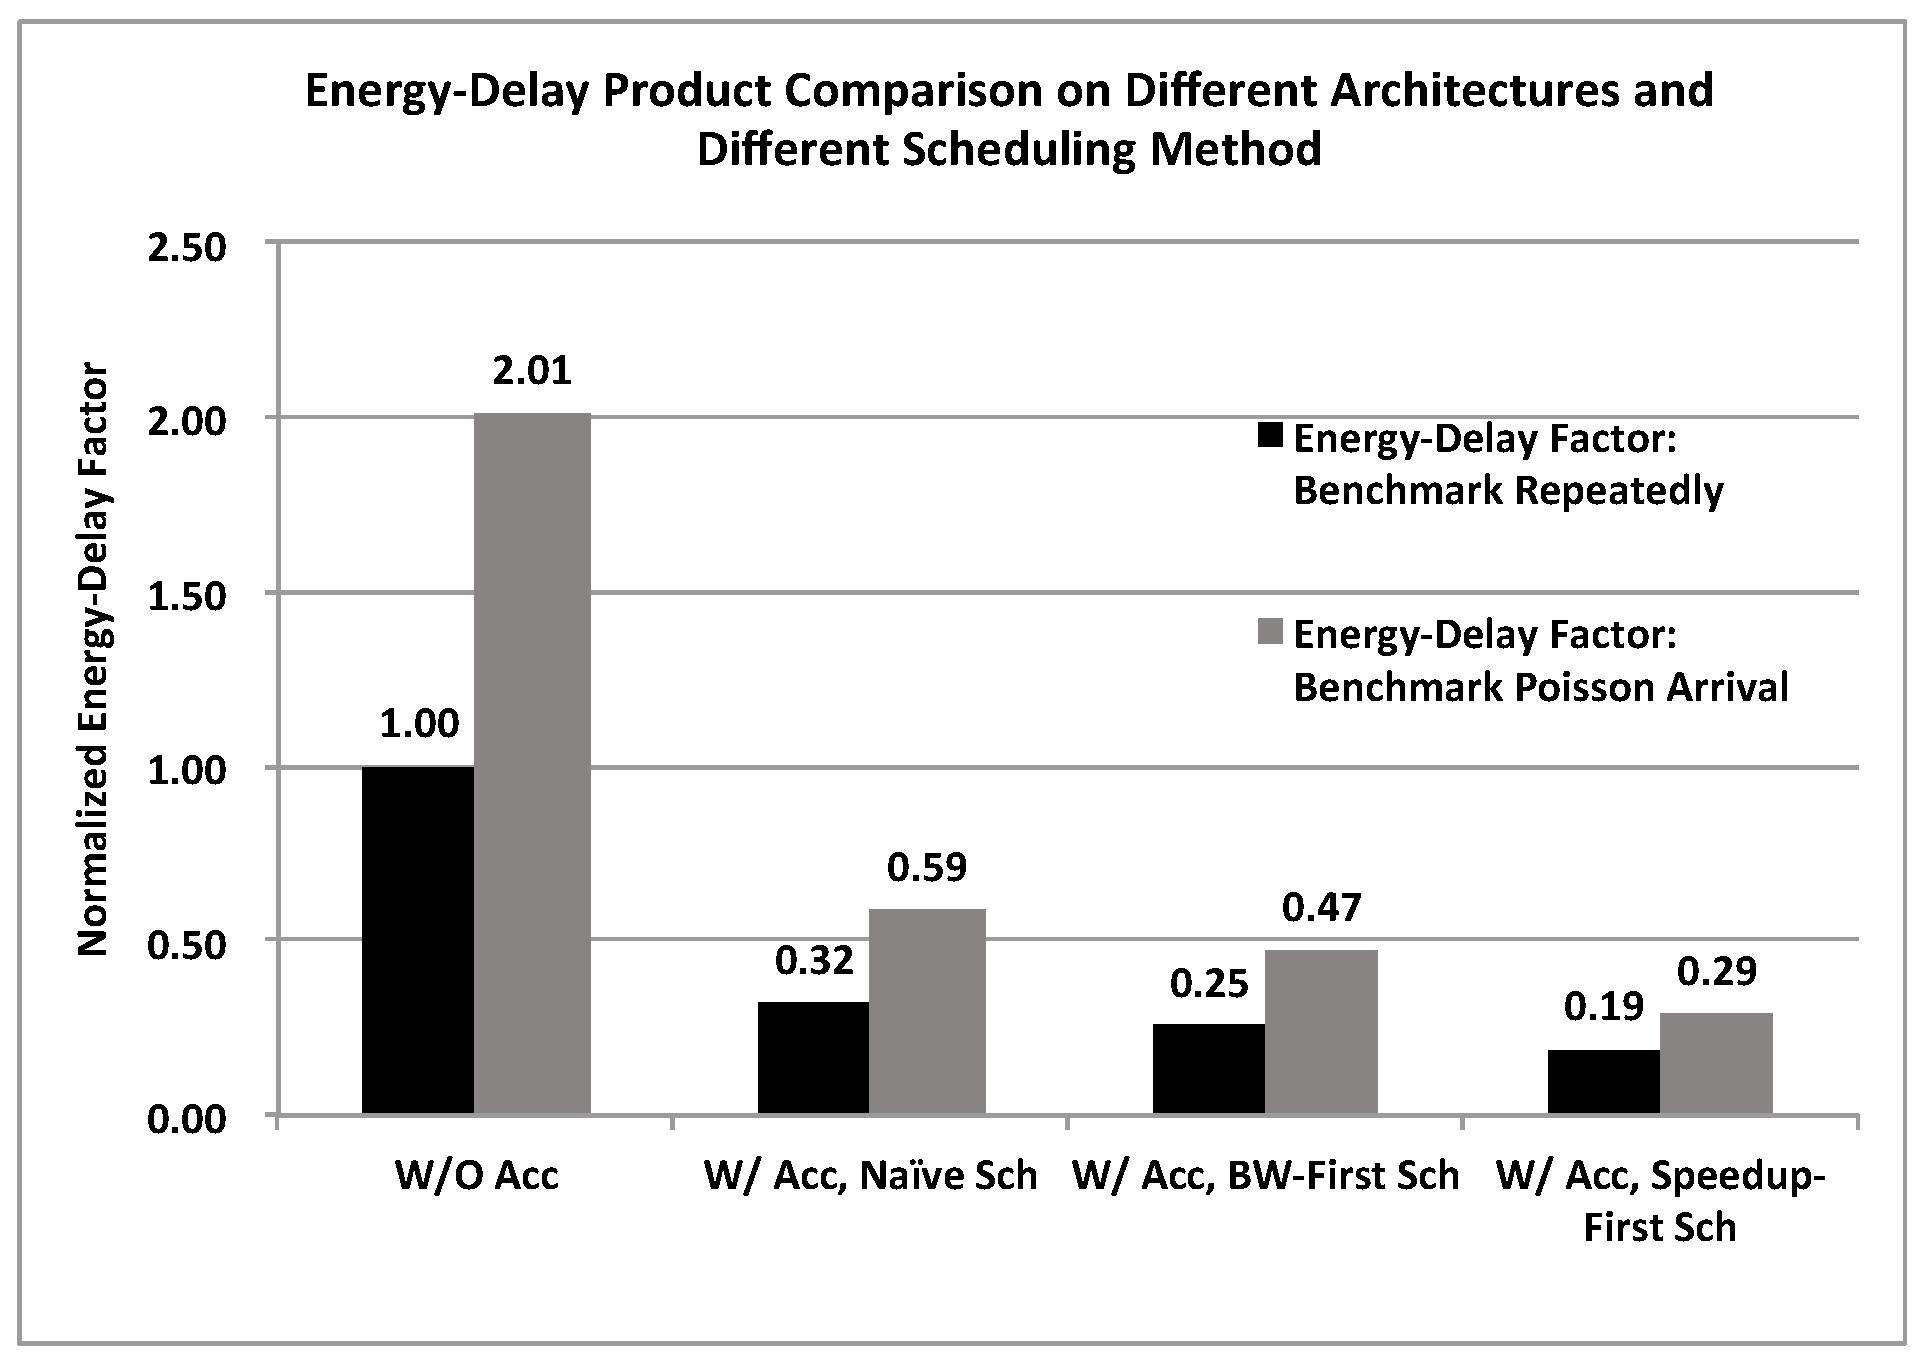
\includegraphics[width=4.5in]{Energy-Delay-8core}
    \caption{Energy-delay Product Comparison.}
    \label{fig_8core_energy_delay}
\end{figure}

In Figure \ref{fig_8core_cycle}, the x-axis denotes different architectures and scheduling methods, such as ``W/O Acc" (without accelerator), ``W/ Acc, 100\% Perfect" (with accelerator and 100\% perfect prediction accuracy of the incoming workloads), ``W/ Acc, Random" (with accelerator and randomly schedule incoming workload to either CPU or accelerators), ``W/ Acc, Acc-First" (with accelerator and schedule workload to accelerators with the first priority), ``W/ Acc, Naive" (with accelerator and profiling only),``W/ Acc, BW-First" (with accelerator and profiling plus Bandwidth First scheduling), and ``W/ Acc, Speedup-First" (with accelerator and Speedup First scheduling). The y-axis stands for the percentage of either performance gain or power efficiency gain.

If not considering the ideal Perfect Prediction scheduling, we can see the accelerated
architectures delivers up to 2.3x improvement on the performance
compared to a multicore architecture without an accelerator. It is
worth noting that such speedup is achieved on a highly dynamic
workload bundle of which the processor has no prior knowledge of the
workload types and arrival times. All the profiling is done at run-time and the
scheduling of the accelerator is autonomously performed by the
middleware (wrapper library). The workload following a Poisson arrival
process has longer execution time because there are idle cycles
between function calls. However, Poisson arrival provides more dynamic
combination of workload arriving at different time, and that's why we
observe a larger speedup (1.46/0.63$\simeq$2.3x) comparing with the
back-to-back arrival (1/0.49$\simeq$2x). 

The energy-delay product depicted in Figure
\ref{fig_8core_energy_delay} show that the power efficiency of {\em
 Transformer} improves by up to (2.01/0.29$\simeq$6.9x) as the workloads migrate to
energy-efficient accelerators due to the scheduling and run-time
reprogramming.

As compared with other different scheduling methods, we also find our profiling methods to be the optimal with the only exception of Perfect Prediction scheduling. For example, the Speedup-First scheduling method outperforms the Random scheduling and Acc-First scheduling with a speedup of 2.12 and 1.96 respectively and a energy-delay factor gain of 5.17 and 4.24 respectively. The results of Perfect Prediction scheduling are promising, however such ``perfect" prediction never happens with the huge dynamics of the workloads in real world. Though ``perfect" in prediction, the Perfect Prediction scheduling method does not yield ``perfect" utilization of the accelerator logics. As we argued in Section \ref{subsec_combo}, maximizing the utilization of reconfigurable logics is one of the contributions in our work to improve system performance and decrease the power consumption. The Bandwidth-First scheduling and the Speedup-First scheduling, on the contrary, take both accelerator size and performance gain into consideration. Thus, on one hand, Bandwidth-First and Speedup-First scheduling methods may not be able to compete with the 100\% Perfect Prediction in terms of the prediction accuracy, however on the other hand, their accelerator combination mechanism improves the whole system performance. As shown in Figure \ref{fig_8core_cycle}, Speedup-First scheduling resembles the performance of the 90\% Perfect Prediction scheduling and Bandwidth-First scheduling matches with the performance of 80\% Perfect Prediction scheduling. 

\subsubsection{Performance and Power Analysis with Various Time Window Sizes}
One of the basic parameter setups of the experiment is the choice of profiling time window $T$. As we mention in \ref{subsec_ranking}, bad choice of $T$ will bring either oversampling or inaccuracy. Thus, we implement a series of experiments to find the optimal range of $T$ that could be used for our benchmarks. 

We take the non-accelerated scenario as the baseline, and compare the performance and power efficiency gain of naive scheduling over the baseline with different profiling time window sizes. The experiment results are shown in Figure \ref{fig_time_window}.

Both performance and power efficiency gain increase when $T$ goes up from $1 ms$ to $100 ms$, stay in the plateau stage when $T$ locates around $100 ms$ to $1000 ms$, and sharply drop when $T$ goes beyond $1000 ms$, where the drop is caused by the accuracy loss of profiling method when down-sampling the benchmarks. According to the results, $[10 ms, 1000 ms]$ is a reasonable range to choose $T$ in our experiment. We also notice that the performance gain and power efficiency gain is still positive when $t = 1 ms$ tough sampling rate is the highest. That means the benefits of applying profiling outperforms the profiling overhead. 

\begin{figure}
    \centering
    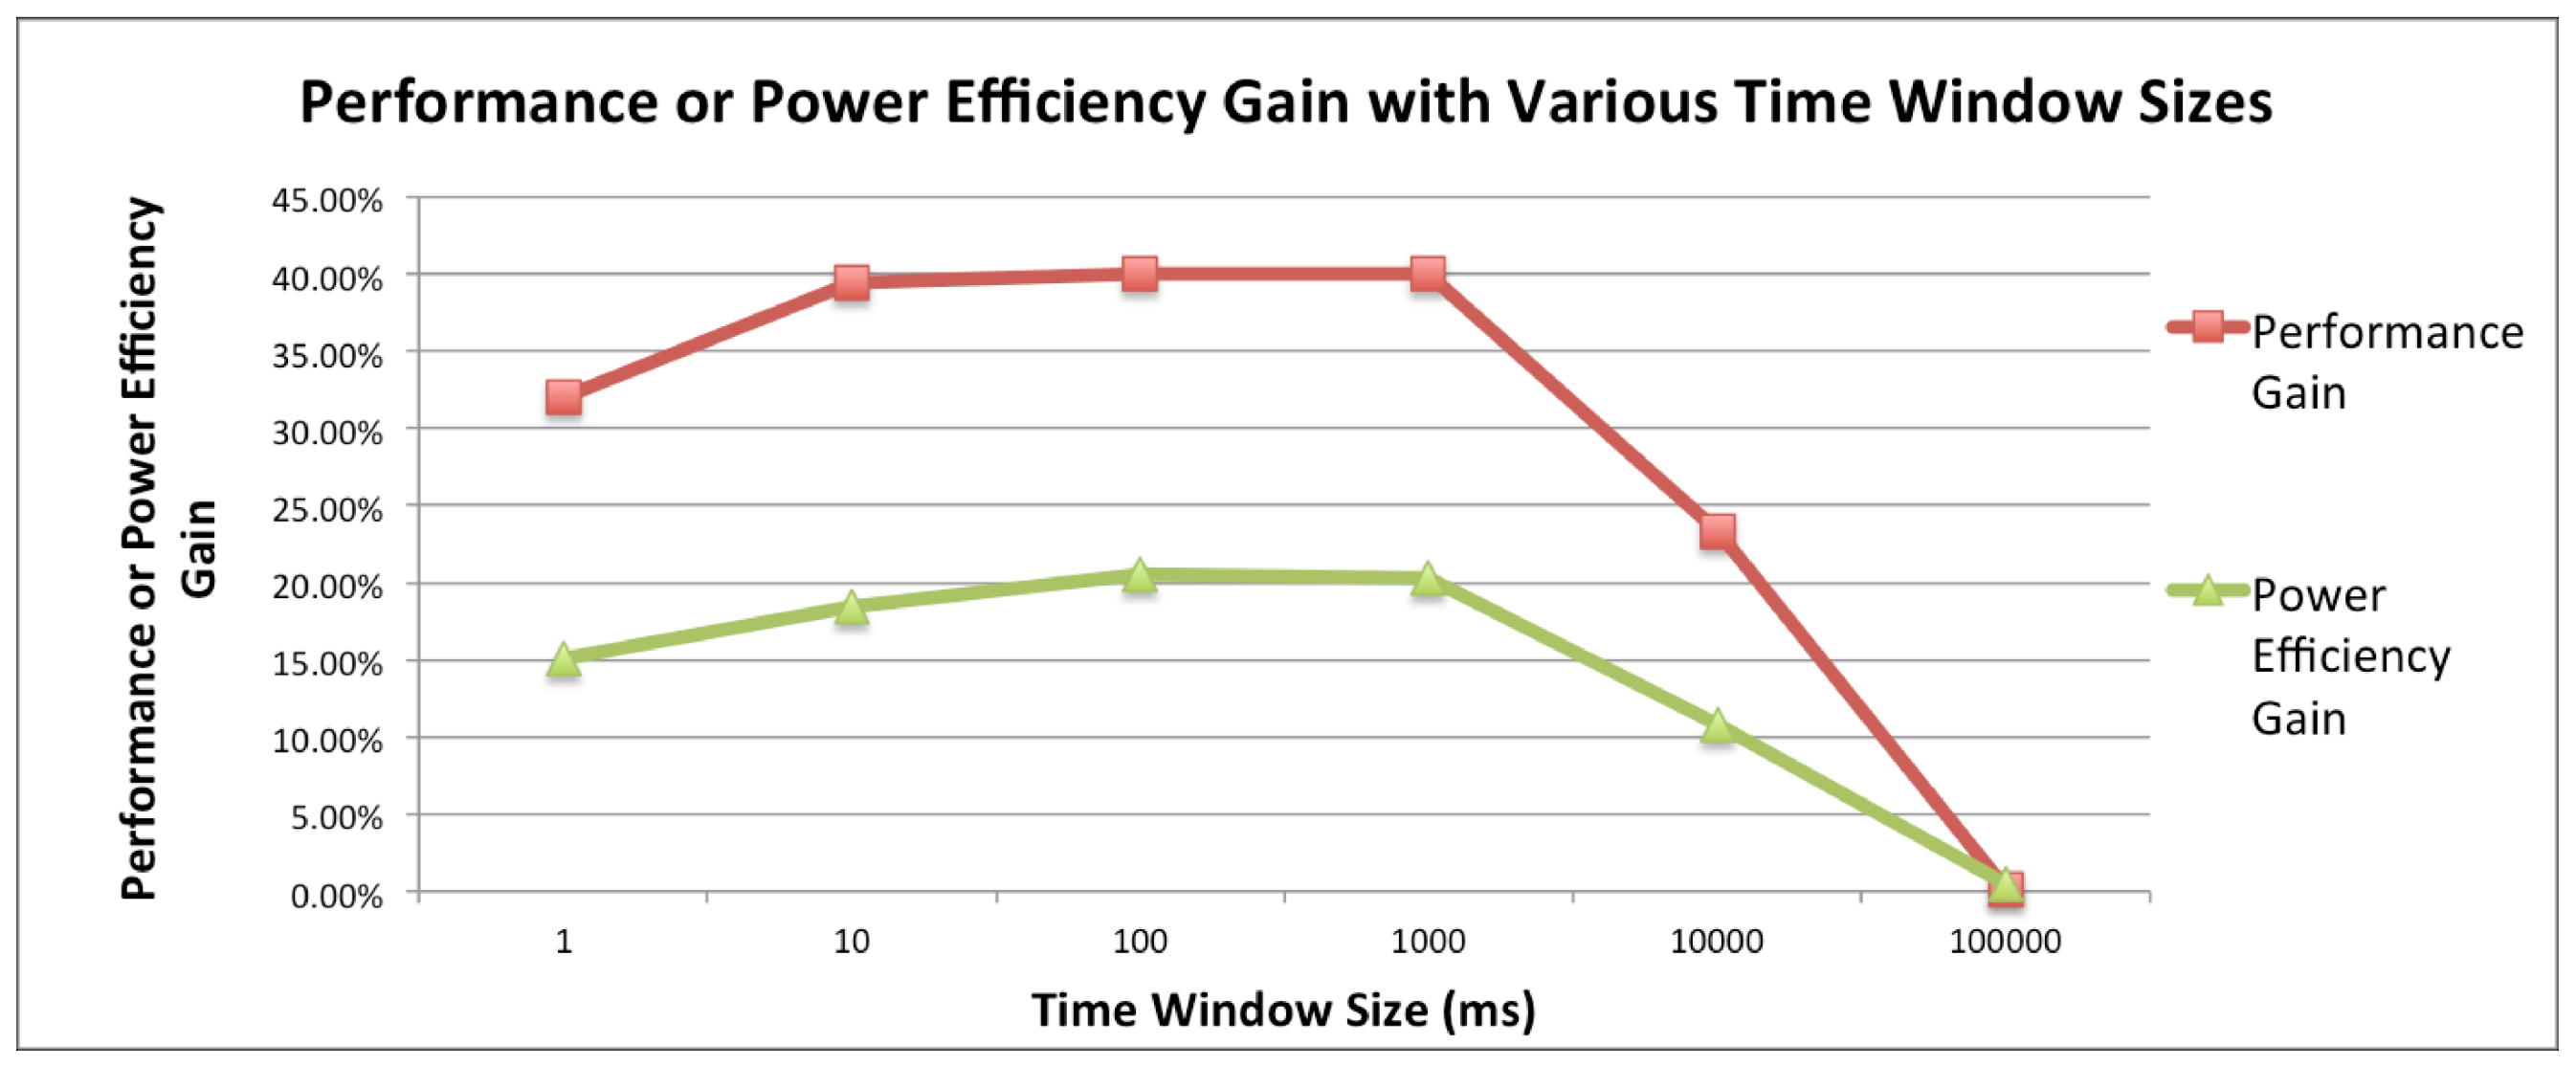
\includegraphics[width=4.5in]{Time-Window-Size}
    \caption{Performance and Power Analysis with Various Time Window Sizes.}
    \label{fig_time_window}
\end{figure}

\subsubsection{Impact of Accelerator Scheduling on Memory-bound vs
  CPU-bound Applications}

We study the impact of the two scheduling heuristics, bandwidth-first
and speedup-first, on different types of workloads, and compare the
heuristics with na\"{\i}ve scheduling (just use calculated priority
rank $P_x$).  We construct two workload bundles based on the memory
access intensity of benchmarks: memory-bound (bandwidth over 500MB/s
in Table \ref{tbl_benchmark}) and CPU-bound.

By design,
bandwidth-first strategy prioritizes the utilization of memory
bandwidth, which inherently gives memory-bandwidth hungry benchmarks
more chances to take advantage of the accelerator logics. As a result,
this strategy outperforms speedup-first for memory-bound
applications as shown in Figure \ref{fig_mem_bound}. On the other hand,
CPU-bound applications benefit more from speedup-first
scheduling strategy as depicted in Figure \ref{fig_cpu_bound}.

\begin{figure}
    \centering
    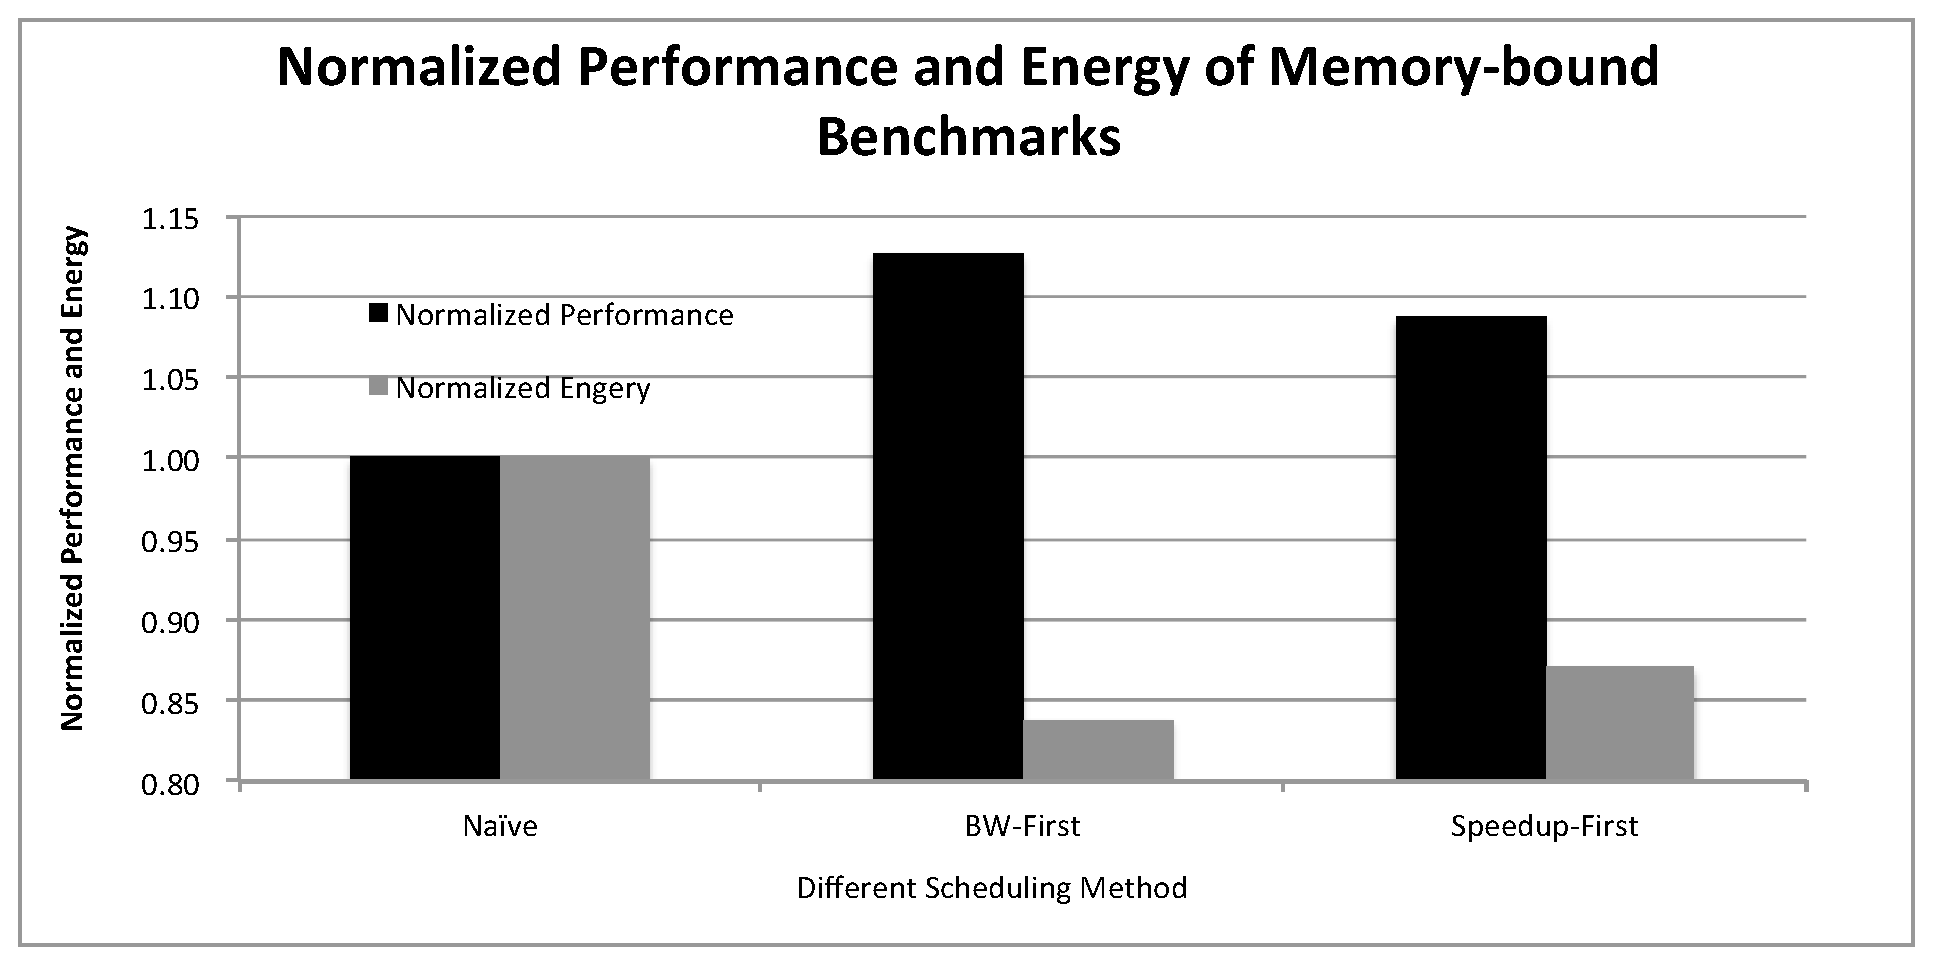
\includegraphics[width=4.5in]{Memory-Bounded}
    \caption{Performance and Energy Consumption of Memory-bound Benchmark Group.}
    \label{fig_mem_bound}
\end{figure}

\begin{figure}
    \centering
    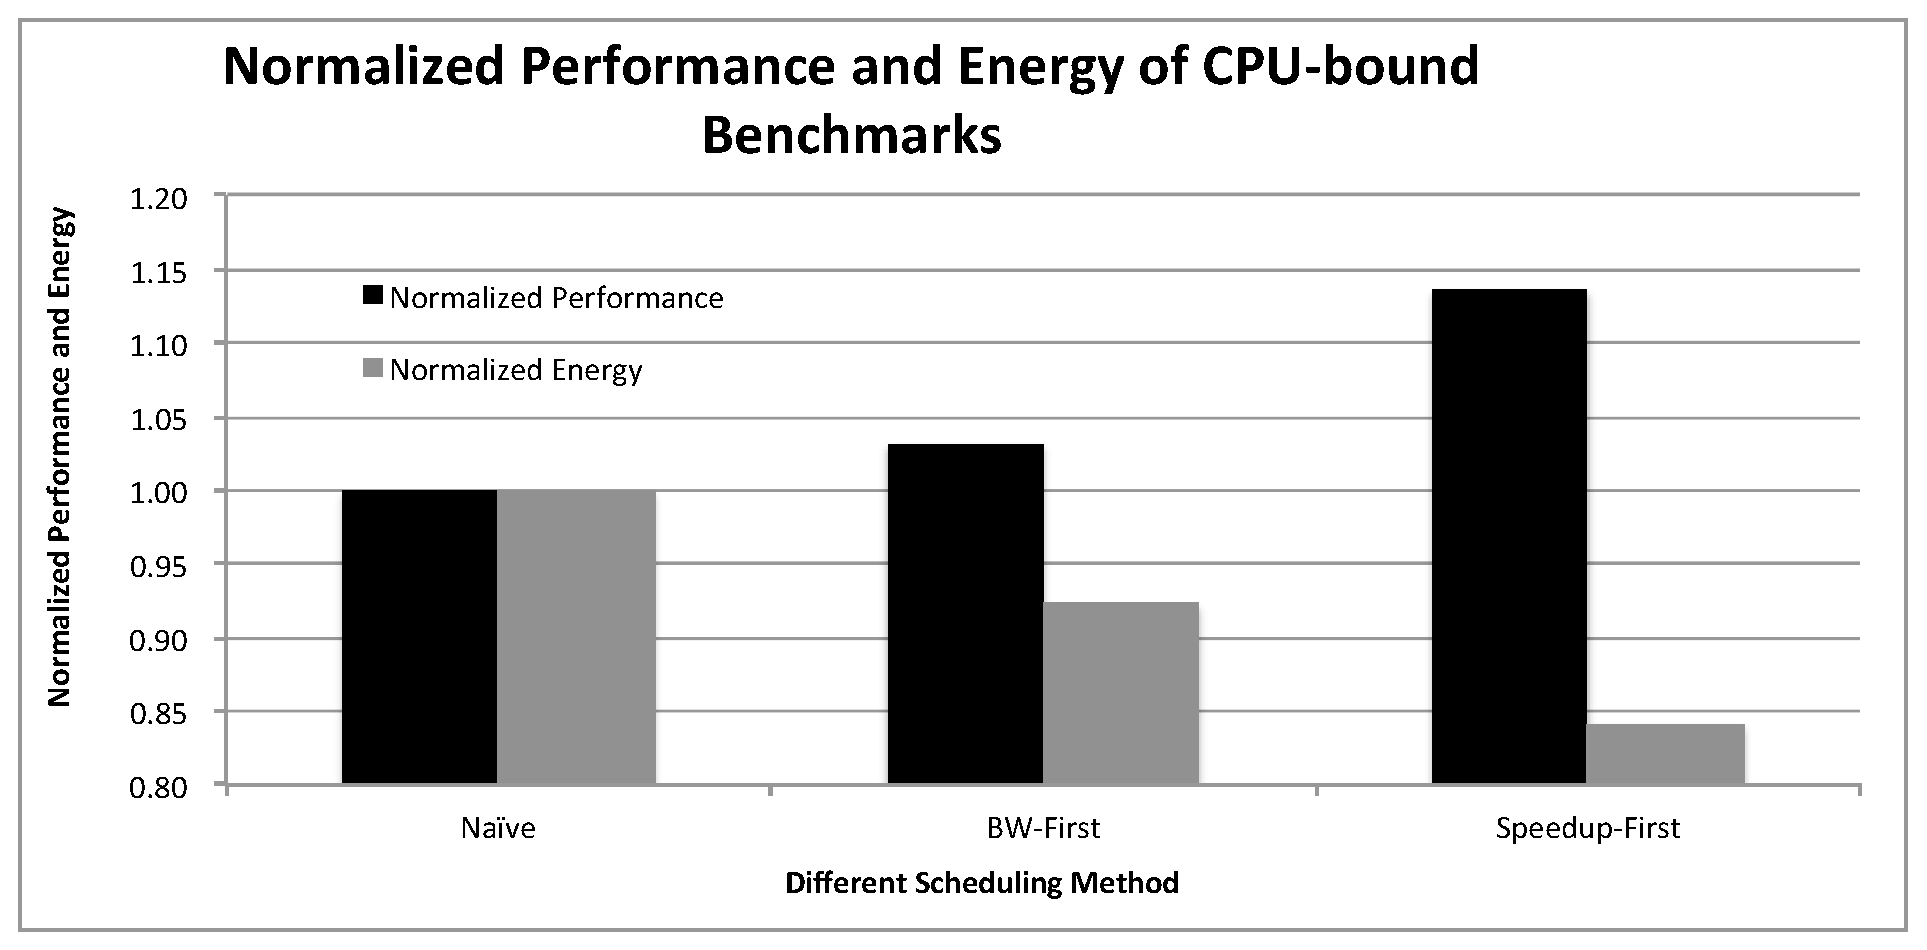
\includegraphics[width=4.5in]{CPU-Bounded}
    \caption{Performance and Energy Consumption on CPU-bound Benchmark Group.}
    \label{fig_cpu_bound}
\end{figure}


\subsubsection{Chip Area Allocation}

It is very interesting to understand how we should allocate chip
area to cores and programmable accelerators, given a limit on the chip
area. We vary the number of cores and the size of the
reconfigurable logic to explore the design space. Figure
\ref{fig_core_acc_ratio} is obtained by changing the core and
accelerator area ratio given a total area equivalent to four cores
plus a Spartan 3E like reconfigurable logic unit (default
accelerator size). As the area of an Atom core is about
    a quarter of Spartan 3E, the combinations of cores and reconfigurable
logics are 8:0, 6:0.5, and so on. It is very interesting to see
 5:0.75 gives the optimal performance gains while more accelerator
logics keep improve the energy efficiency. While such ratio is
specific to the workloads and should be cautiously generalized, 
our results show that it is important to
investigate the design space to explore the best possible
combinations of cores and accelerators. 

\begin{figure}
    \centering
    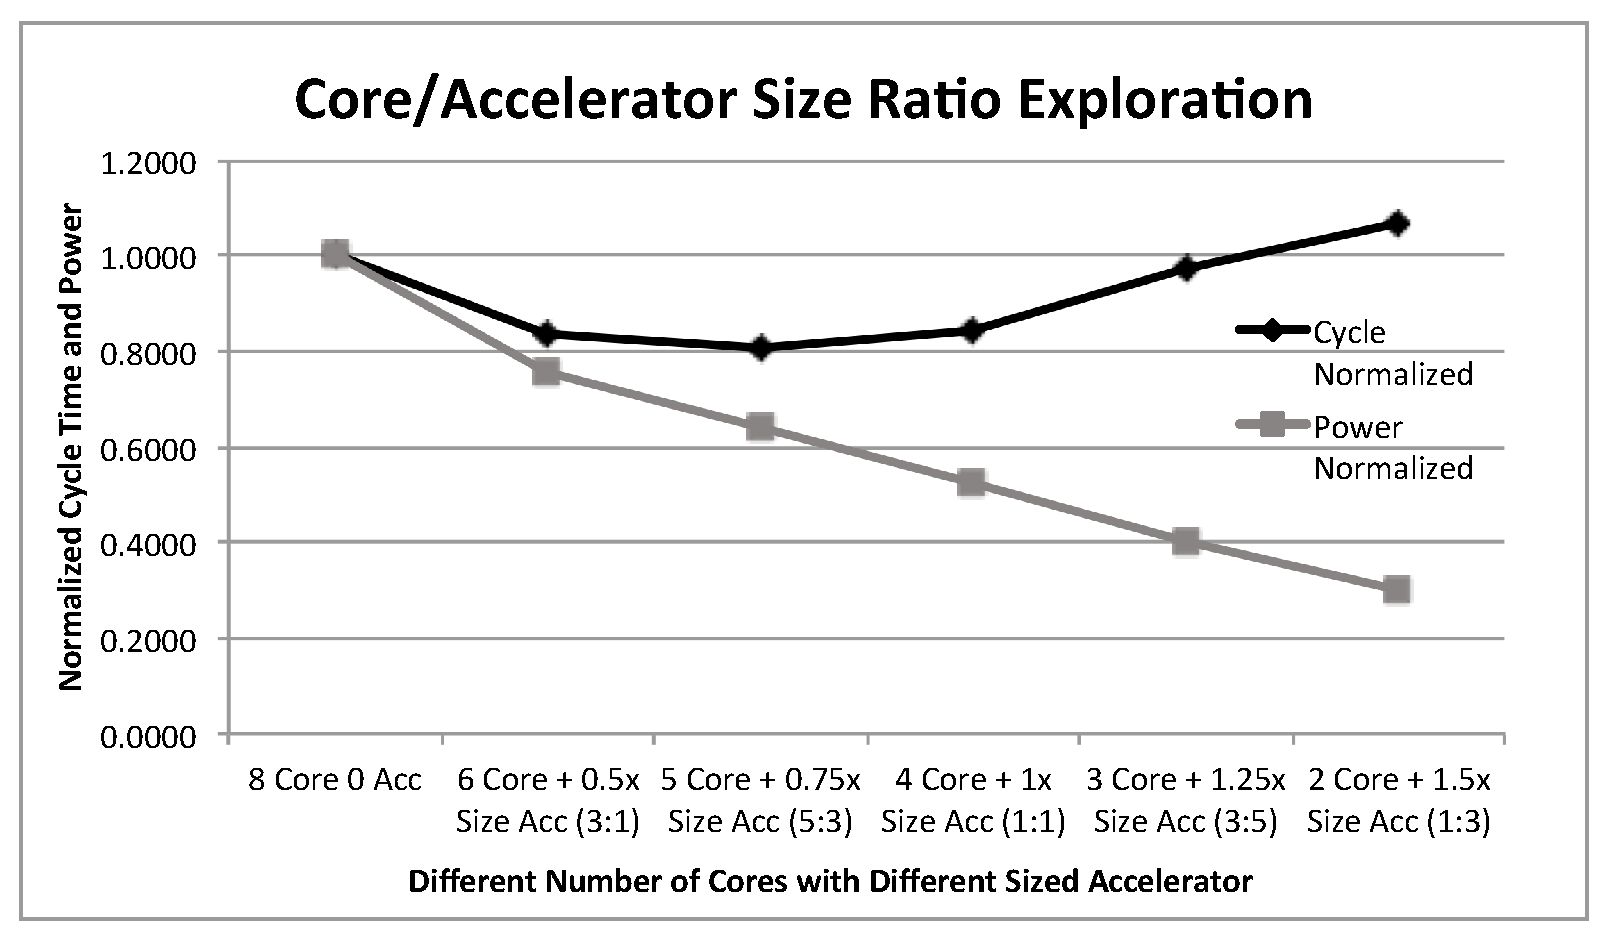
\includegraphics[width=4.5in]{Core-Acc-Size-Ratio}
    \caption{Performance and Power with Different Core/Accelerator Ratios.}
    \label{fig_core_acc_ratio}
\end{figure}

\subsubsection{Experiment Parameter Analysis}
One of the contributions of this work is to provide insights into how different parameters of the heterogeneous architecture or the benchmark will affect the performance and power efficiency on the heterogeneous architecture. Thus, we study the same performance and energy efficiency metrics with different architecture parameters to render better understandings of choosing parameters. 

Cache is becoming the number one area and power consuming component on a CMP system. Thus, we first study L1 cache size as shown in Figure \ref{fig_l1_perf}. Our system prototyped L1 cache size is 32 KB, thus 32 KB L1 cache with naive scheduling is considered as the baseline in this experiment. The performance gain increases fast when L1 cache size changes from 8 KB to 32 KB - around 12\% to 14\%; however the increase slows down when cache size changes beyond 32 KB. This result means that 32 KB of L1 cache is relatively large enough for our benchmarks. Power efficiency, on the other hand, drops steadily when cache size increases as shown in Figure \ref{fig_l1_power}. This is because the increase of cache size will great impact both static and dynamic power. 

We conduct a similar experiment with change of L2 cache size in Figure \ref{fig_l2_perf} and \ref{fig_l2_power}. When we increase the size of L2 cache, both the performance gain and power efficiency gain increase or decrease with a steady rate. However, the slope of the gain is much higher than that in L1 cache's results. That is partially because accelerators and CPUs share the L2 cache with MOESI coherence. So when cache size increases, the heterogeneous architecture benefits from the lower rate of cache miss. 

Accelerator local buffer works similarly as core's L1 cache. Thus, the characteristics of accelerator local buffer resemble with L1 cache's curves as shown in Figure \ref{fig_acc_buffer_perf} and \ref{fig_acc_buffer_power}. The only difference is that when we gradually change the buffer size, the gain changing rate of local buffer is higher than that of L1 cache. This is because the hardware implementation is more sensitive to the locality of input data since there is more data parallelism in accelerators. 

We also study the inter-arrival time of the Poisson-distributed benchmark mixture to find if the dynamics of the workload will affect the system performance. As illustrated in Figure \ref{fig_benchmark-switching}, we take the 500 million cycles inter-arrival time with naive scheduling as the baseline since ``500 million cycles" is the setup in our experiment. The tendency of the performance gain is dropping when the benchmark inter-arrival time varies from 0 cycle to 1000 million cycles. When inter-arrival time is equal to 0, it is identical with the back-to-back setup of workload. This figure demonstrates that the more frequent change of benchmarks in the workload, the more precise of the profiling-prediction could be, and the more benefit we can gain from the scheduling methods though the overhead of accelerator reprogramming is also increasing. In addition, the performance gain difference is becoming larger between the naive scheduling methods and the other two methods when inter-arrival time increases. This is because the prediction benefit is mitigated when inter-arrival time becomes too large, however, BW-First and Speedup-First scheduling still benefit from accelerator combining. 

\begin{figure}
    \centering
    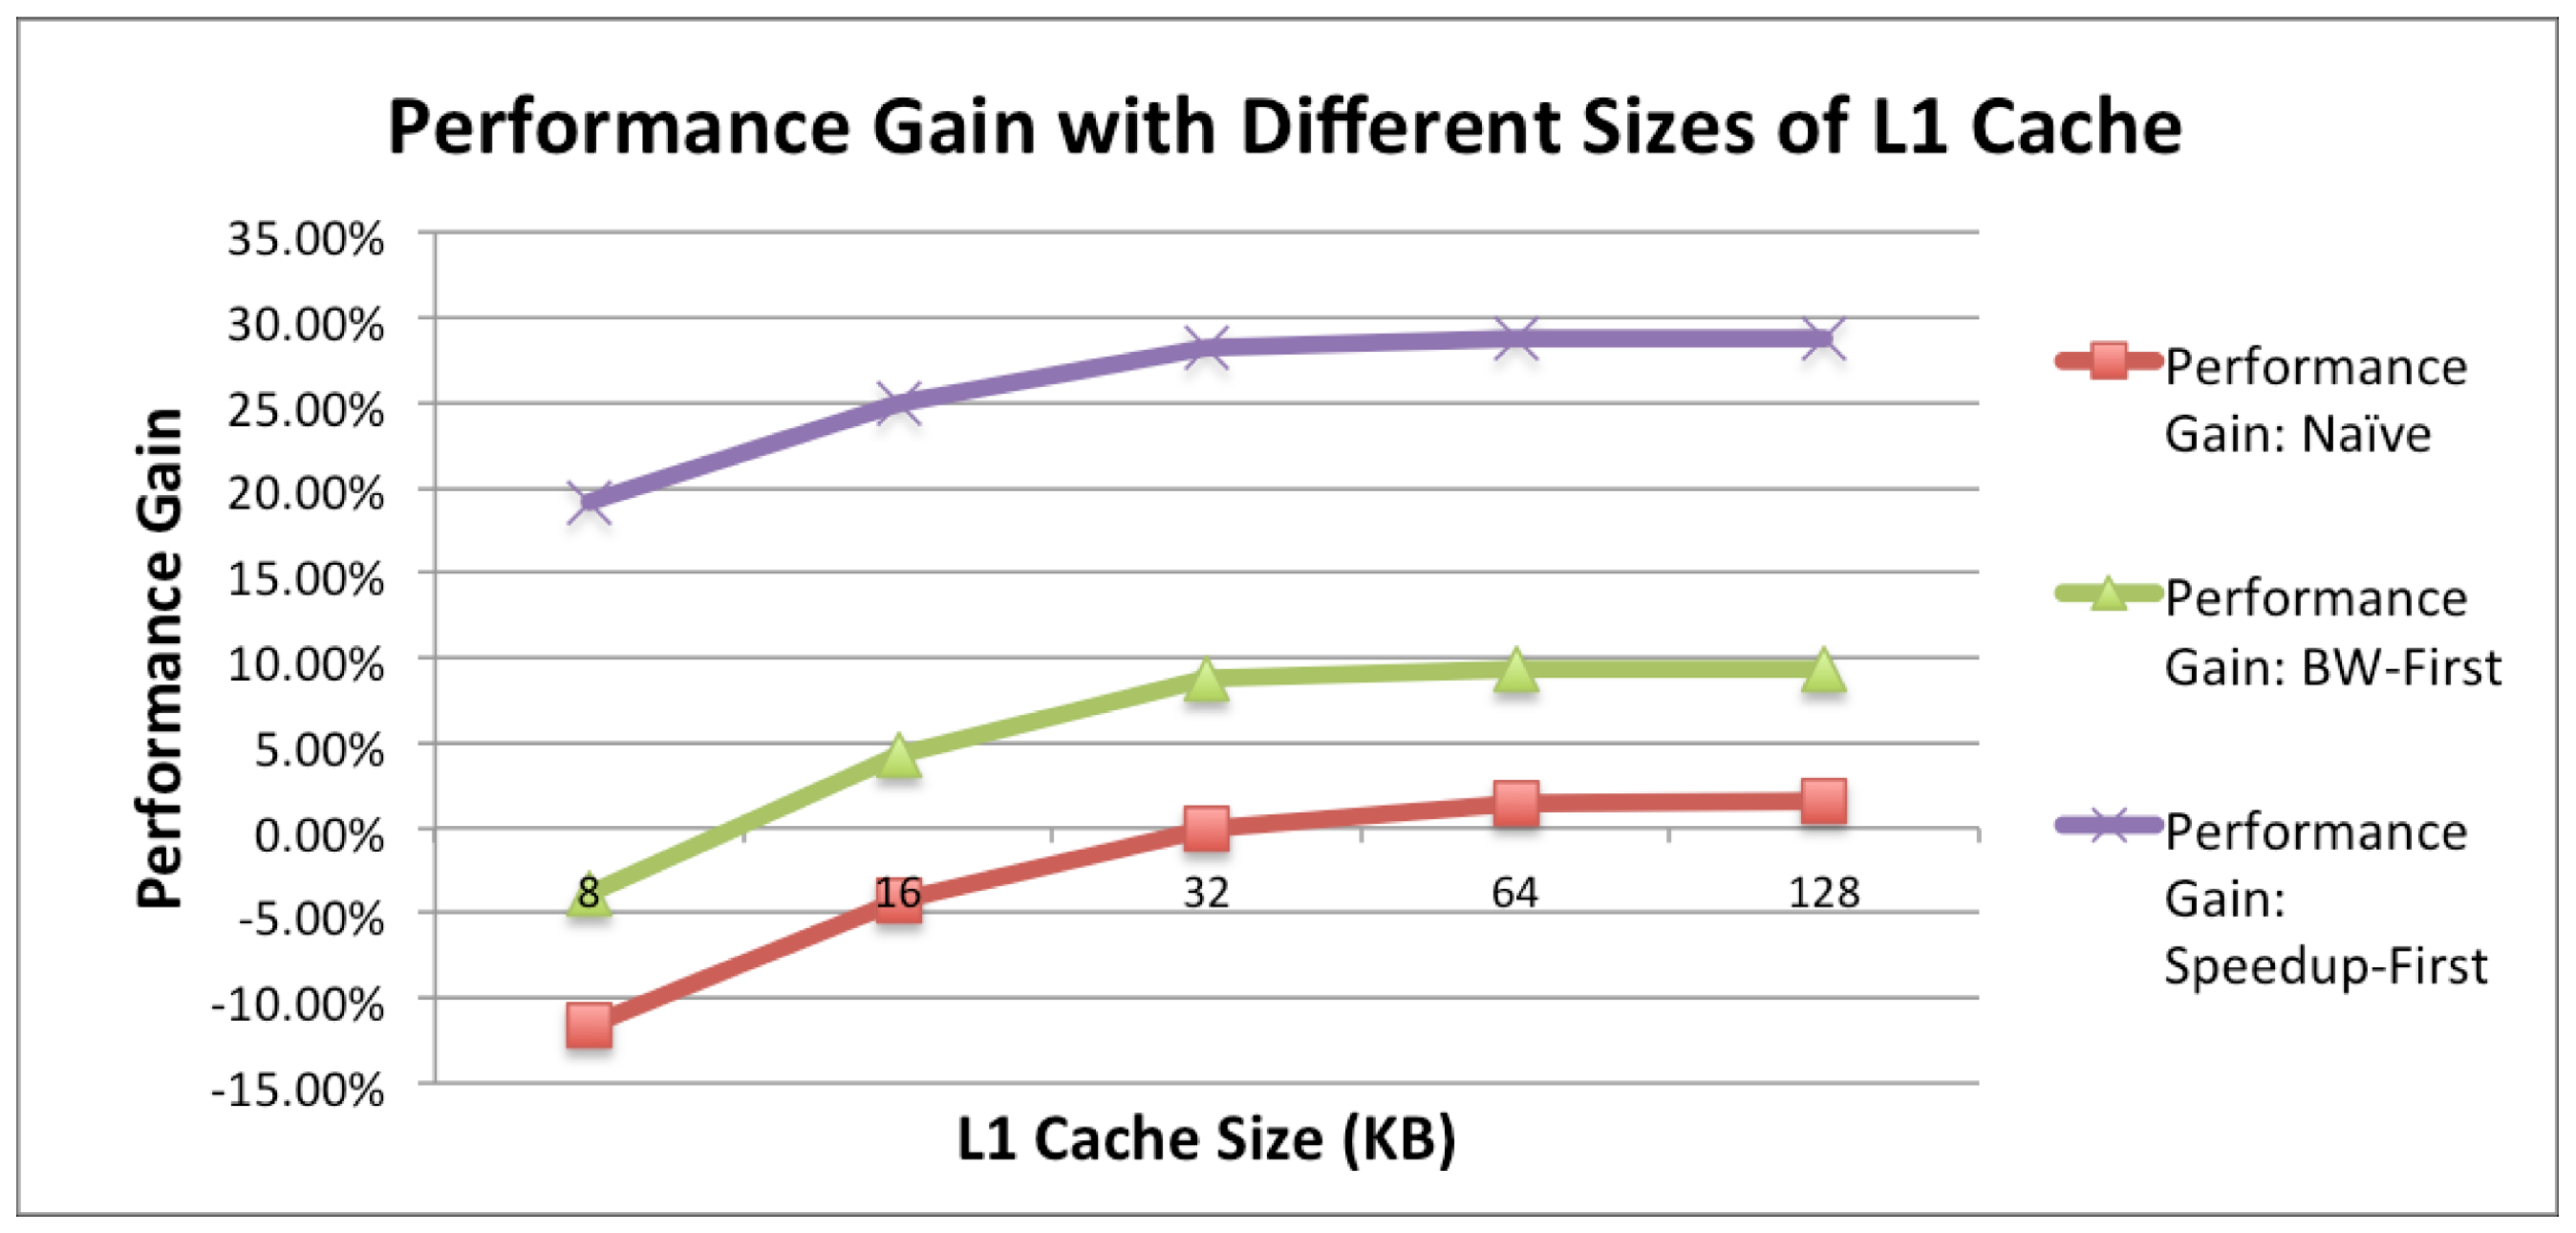
\includegraphics[width=4.5in]{L1-Cache-Performance}
    \caption{Performance Gain with Different Sizes of L1 Cache.}
    \label{fig_l1_perf}
\end{figure}

\begin{figure}
    \centering
    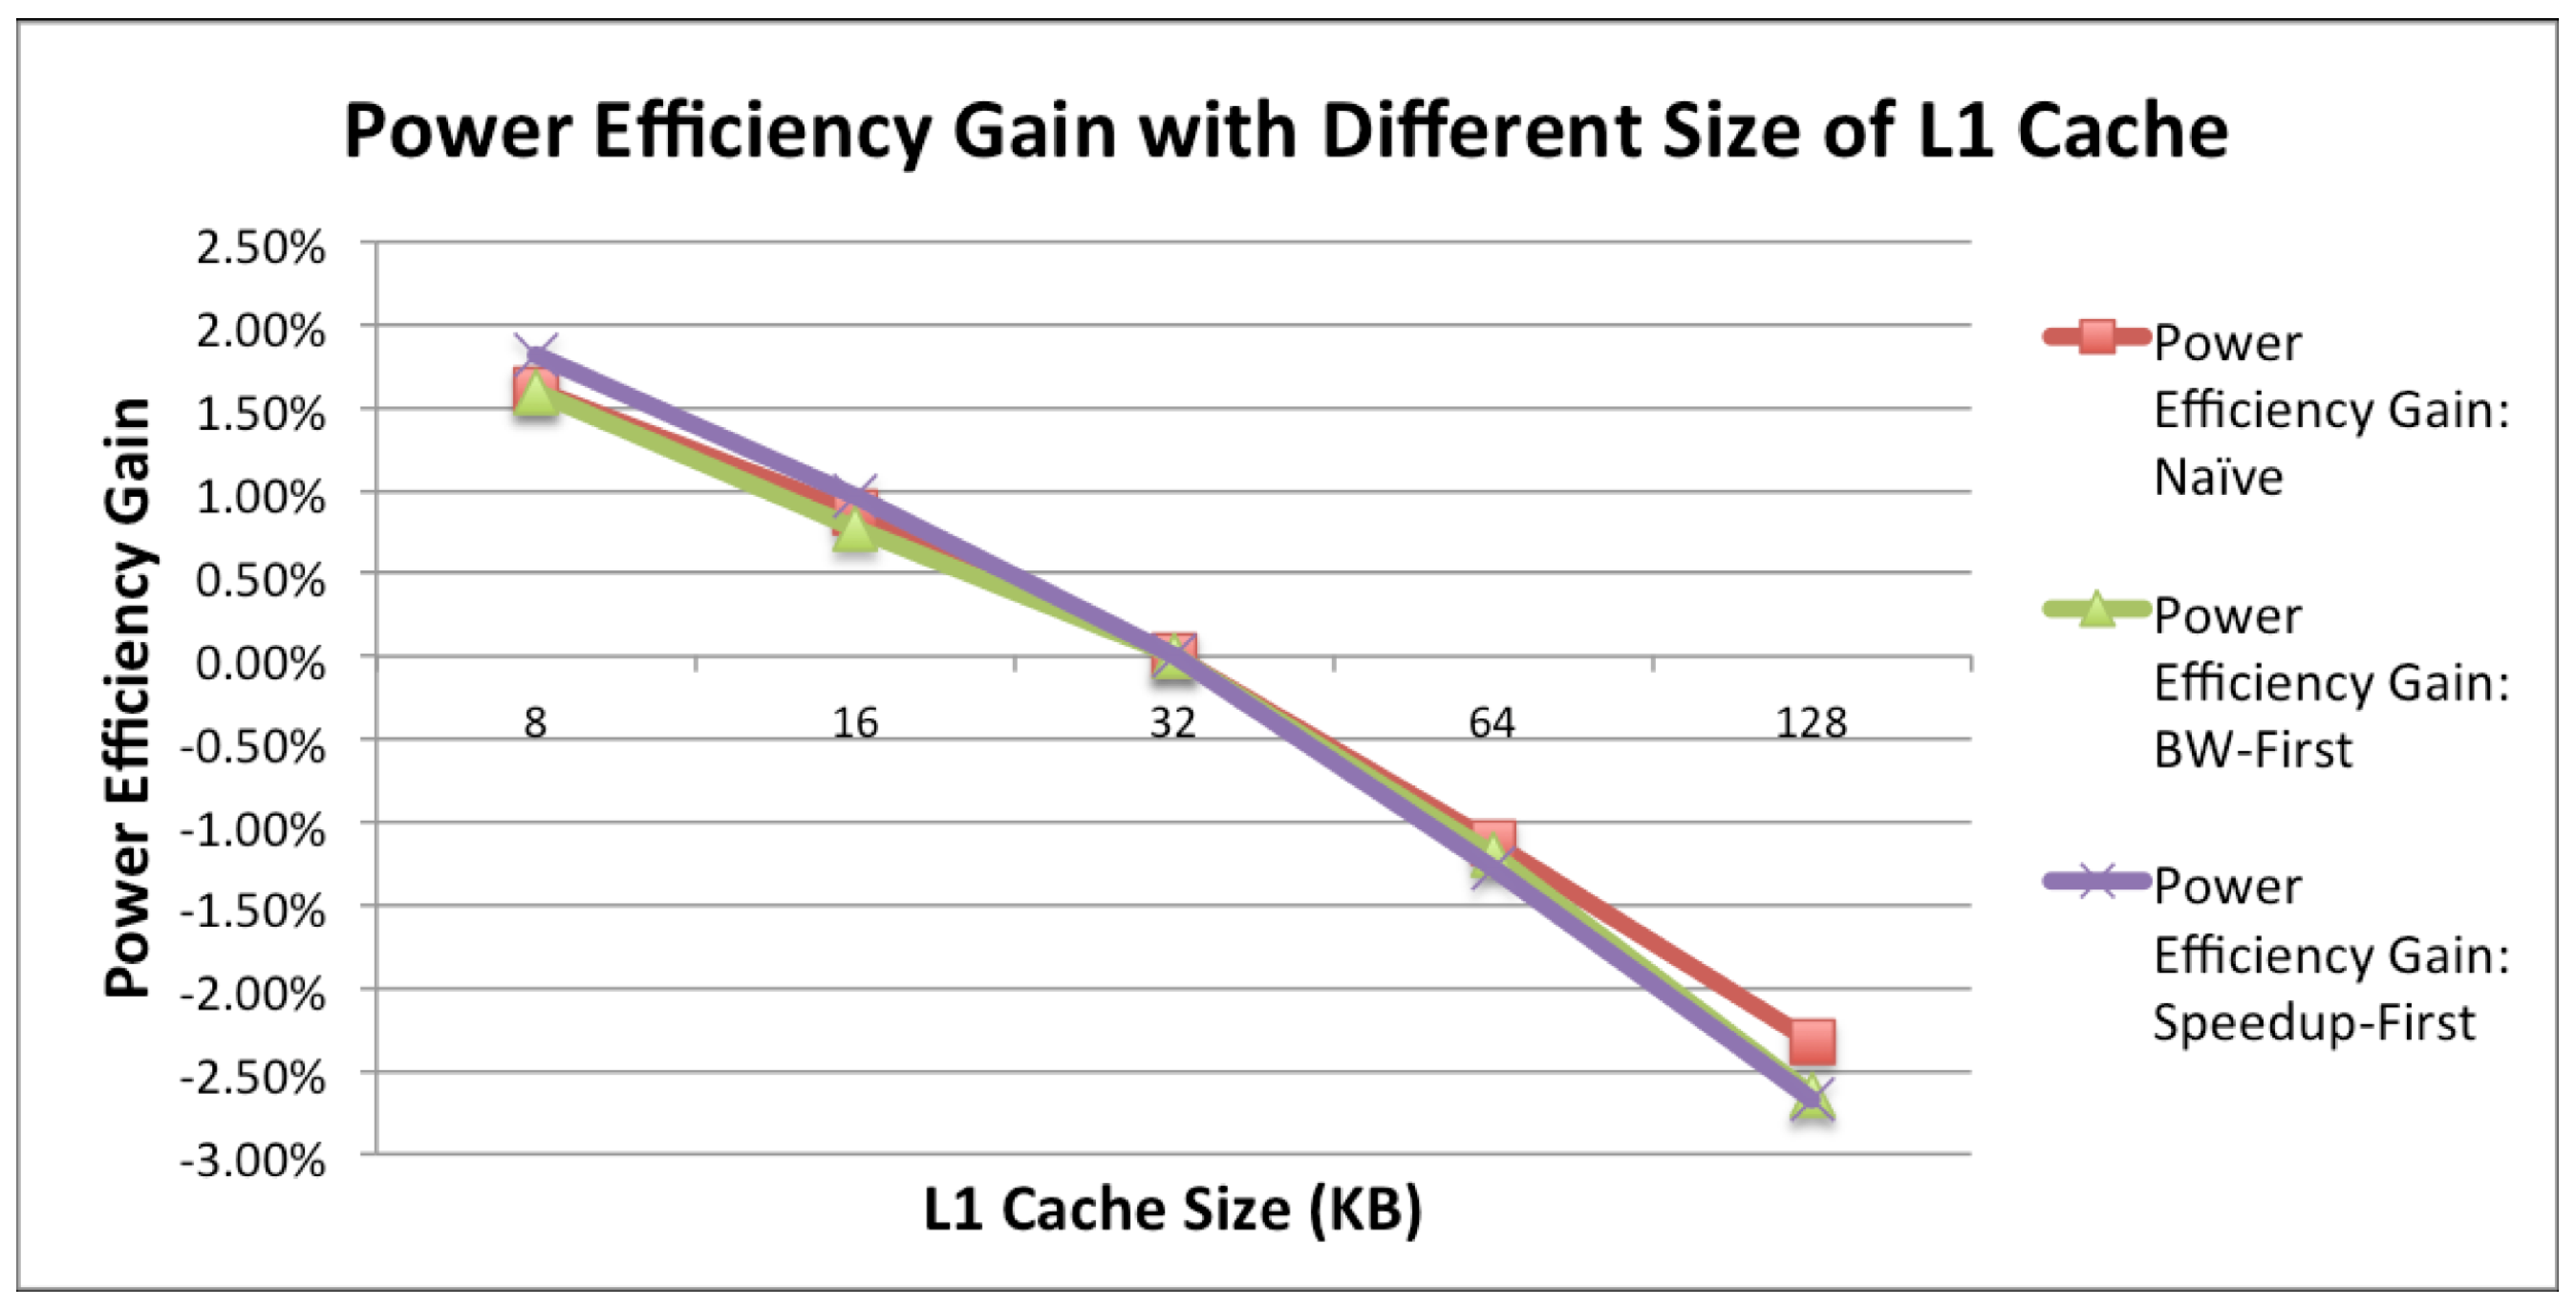
\includegraphics[width=4.5in]{L1-Cache-Power}
    \caption{Power Efficiency Gain with Different Sizes of L1 Cache.}
    \label{fig_l1_power}
\end{figure}

\begin{figure}
    \centering
    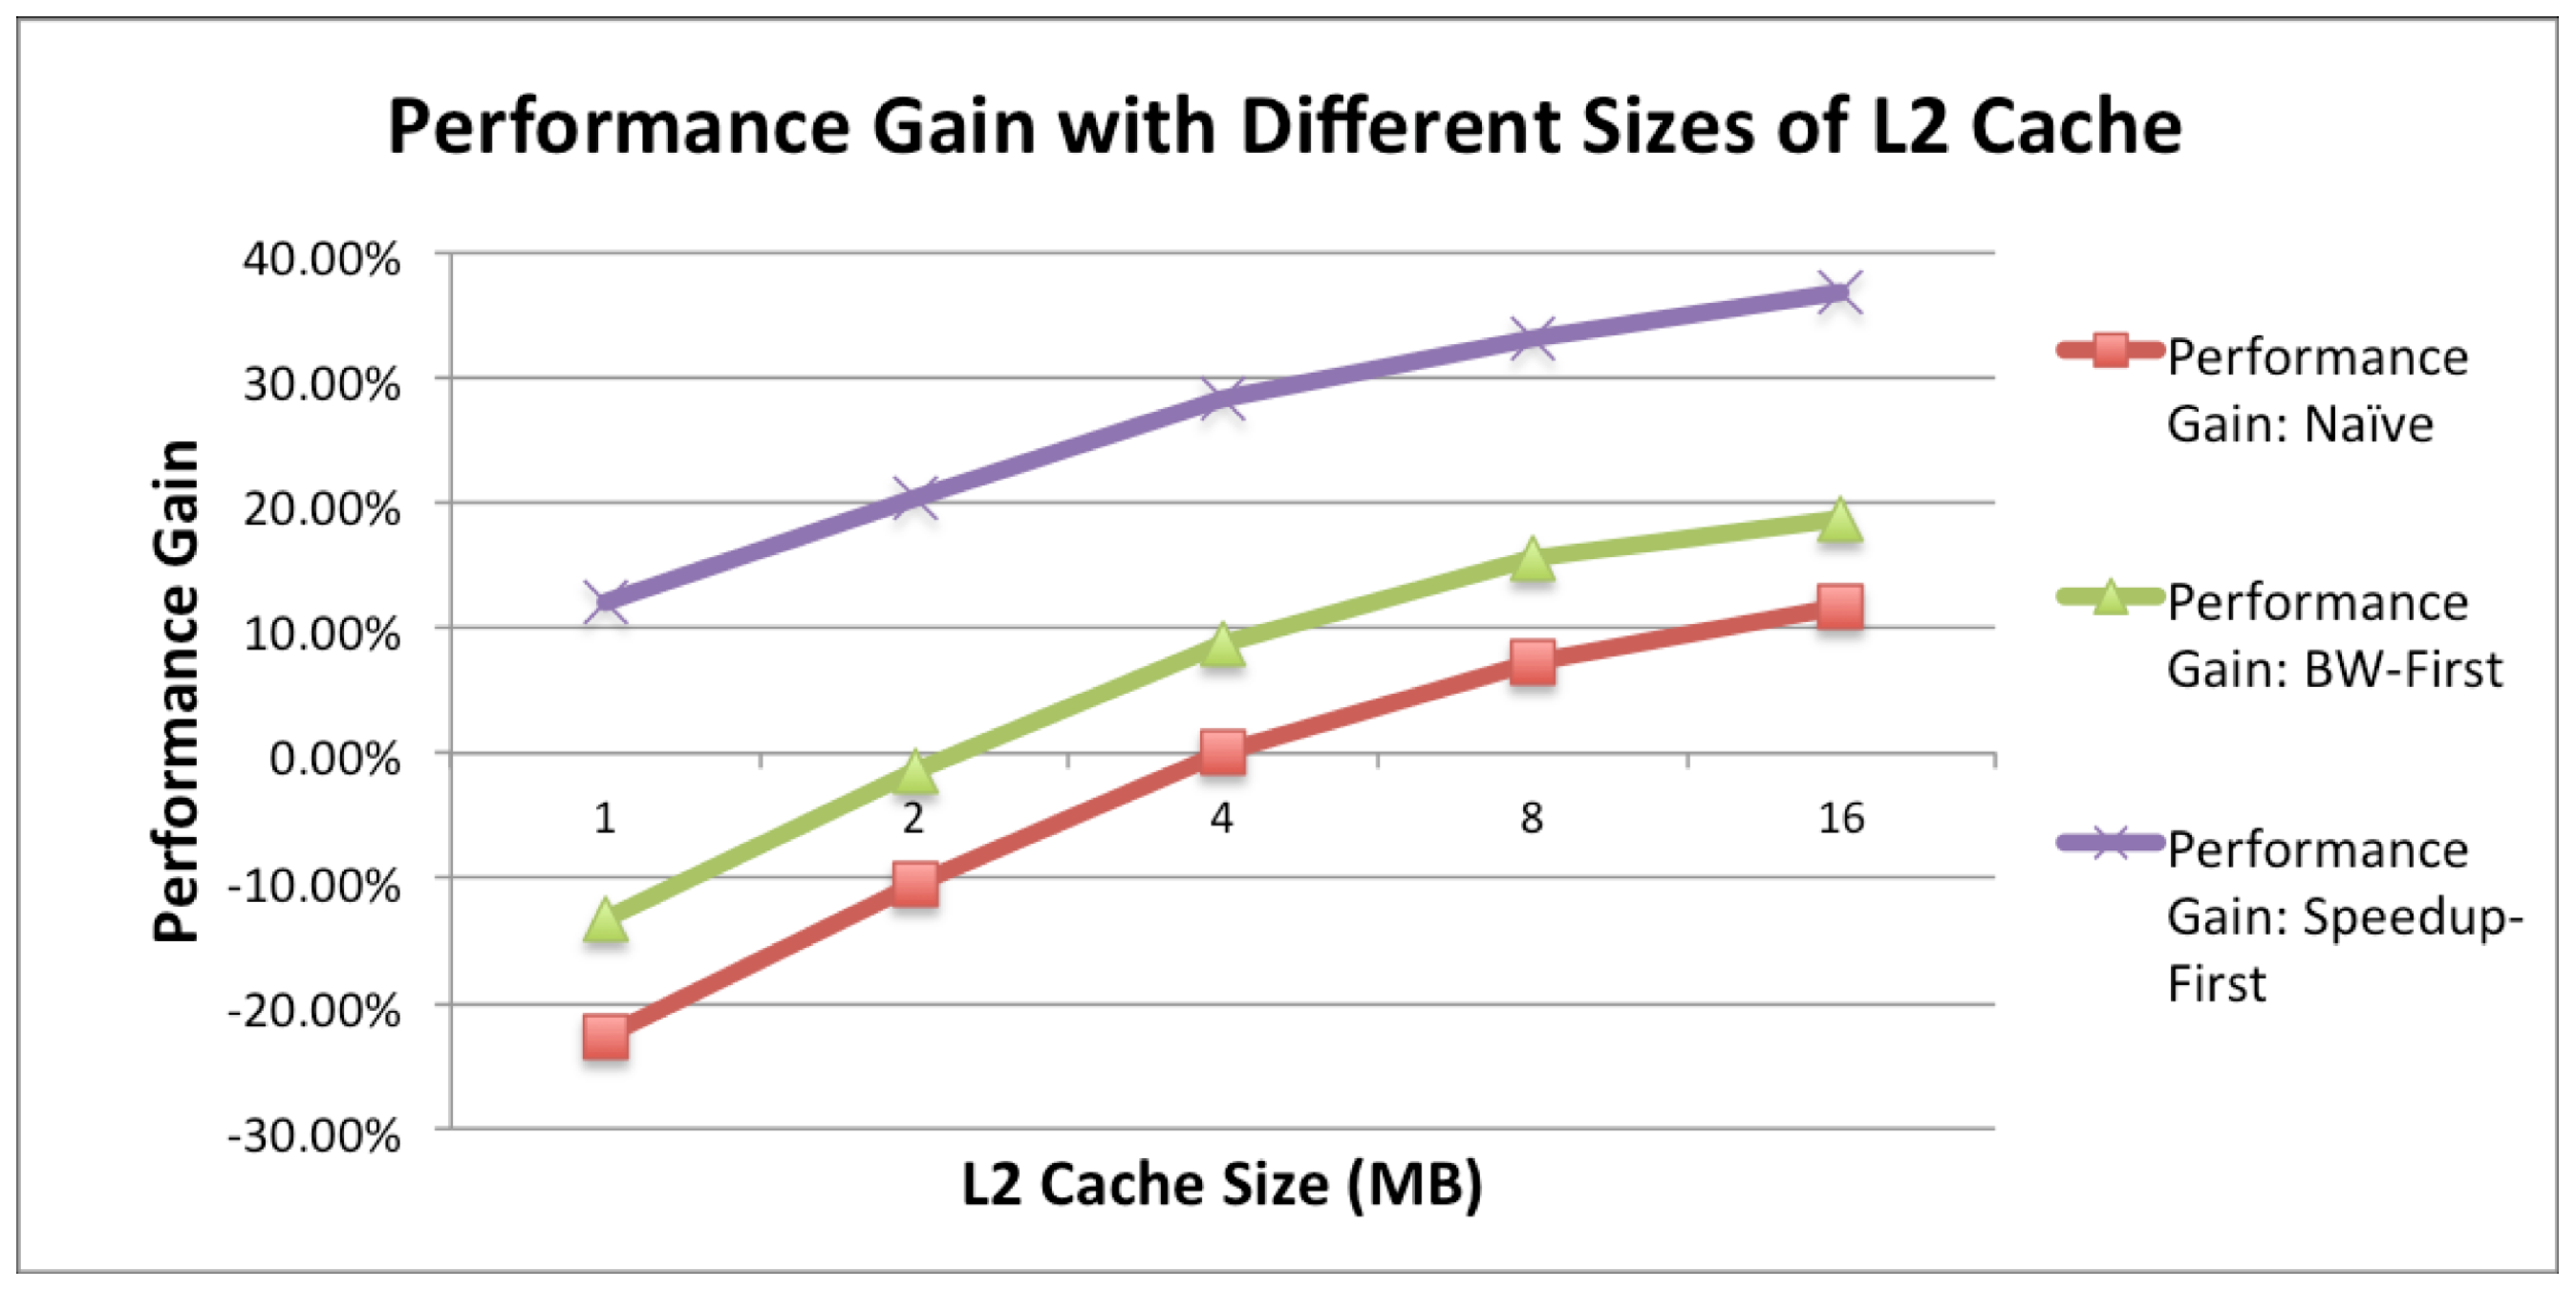
\includegraphics[width=4.5in]{L2-Cache-Performance}
    \caption{Performance Gain with Different Sizes of L2 Cache.}
    \label{fig_l2_perf}
\end{figure}

\begin{figure}
    \centering
    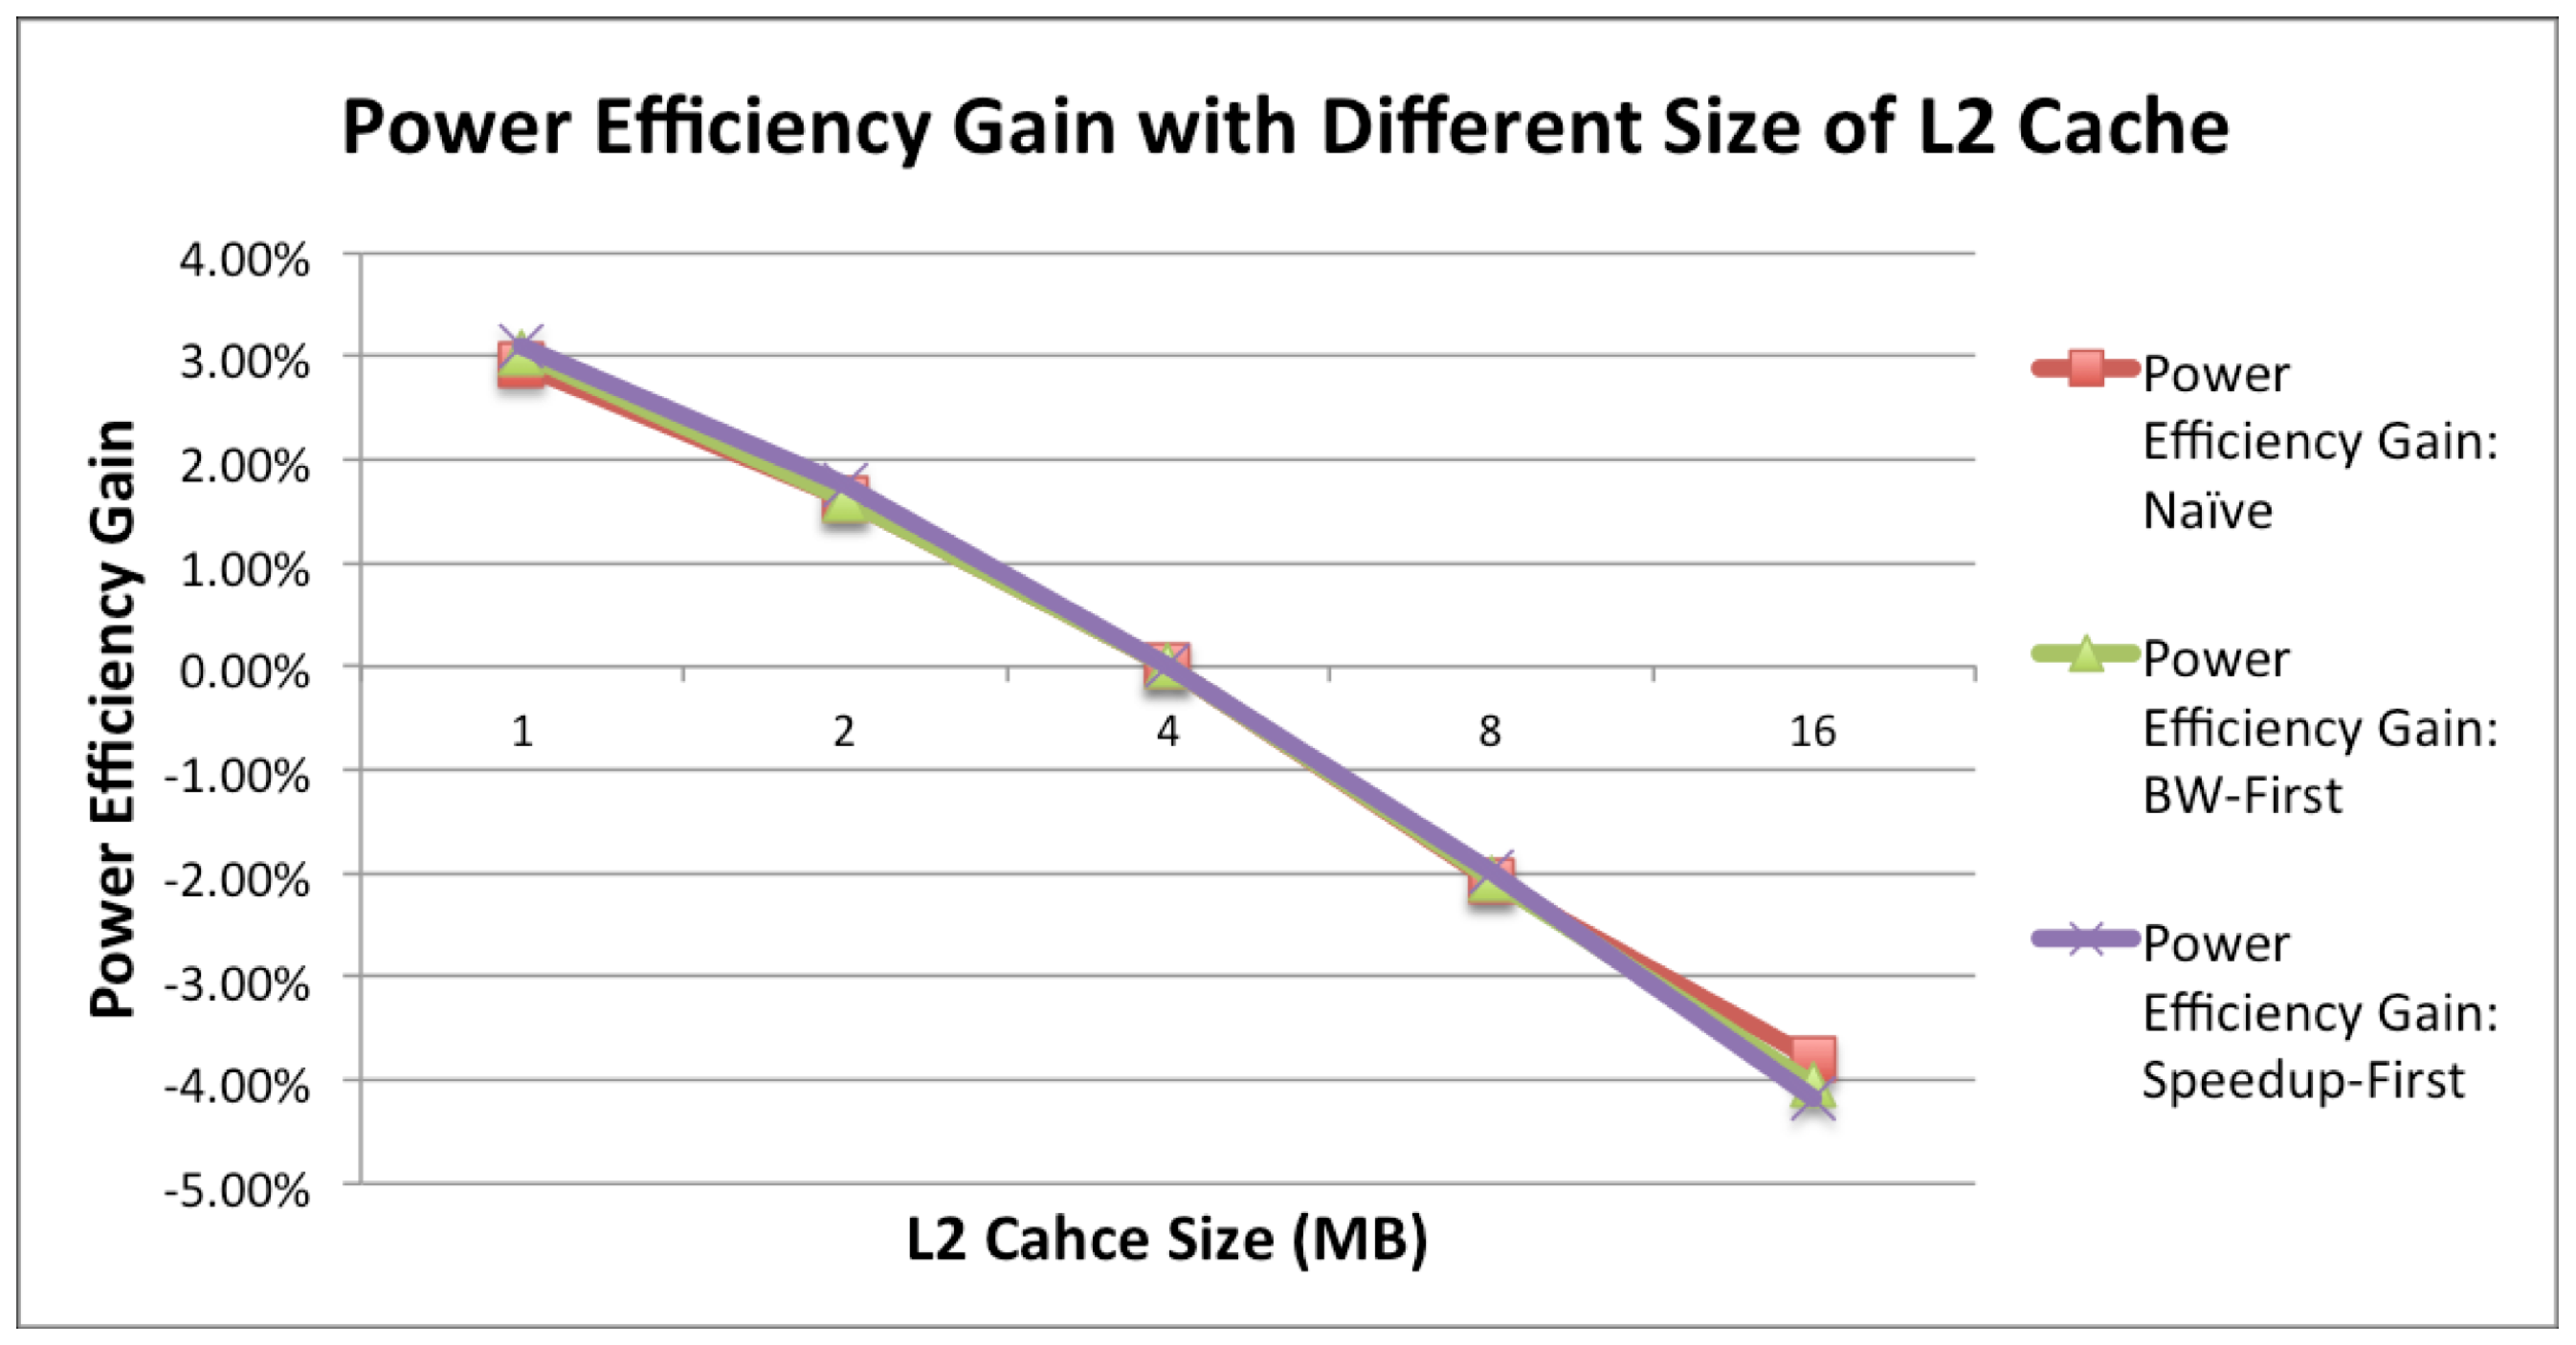
\includegraphics[width=4.5in]{L2-Cache-Power}
    \caption{Power Efficiency Gain with Different Sizes of L2 Cache.}
    \label{fig_l2_power}
\end{figure}

\begin{figure}
    \centering
    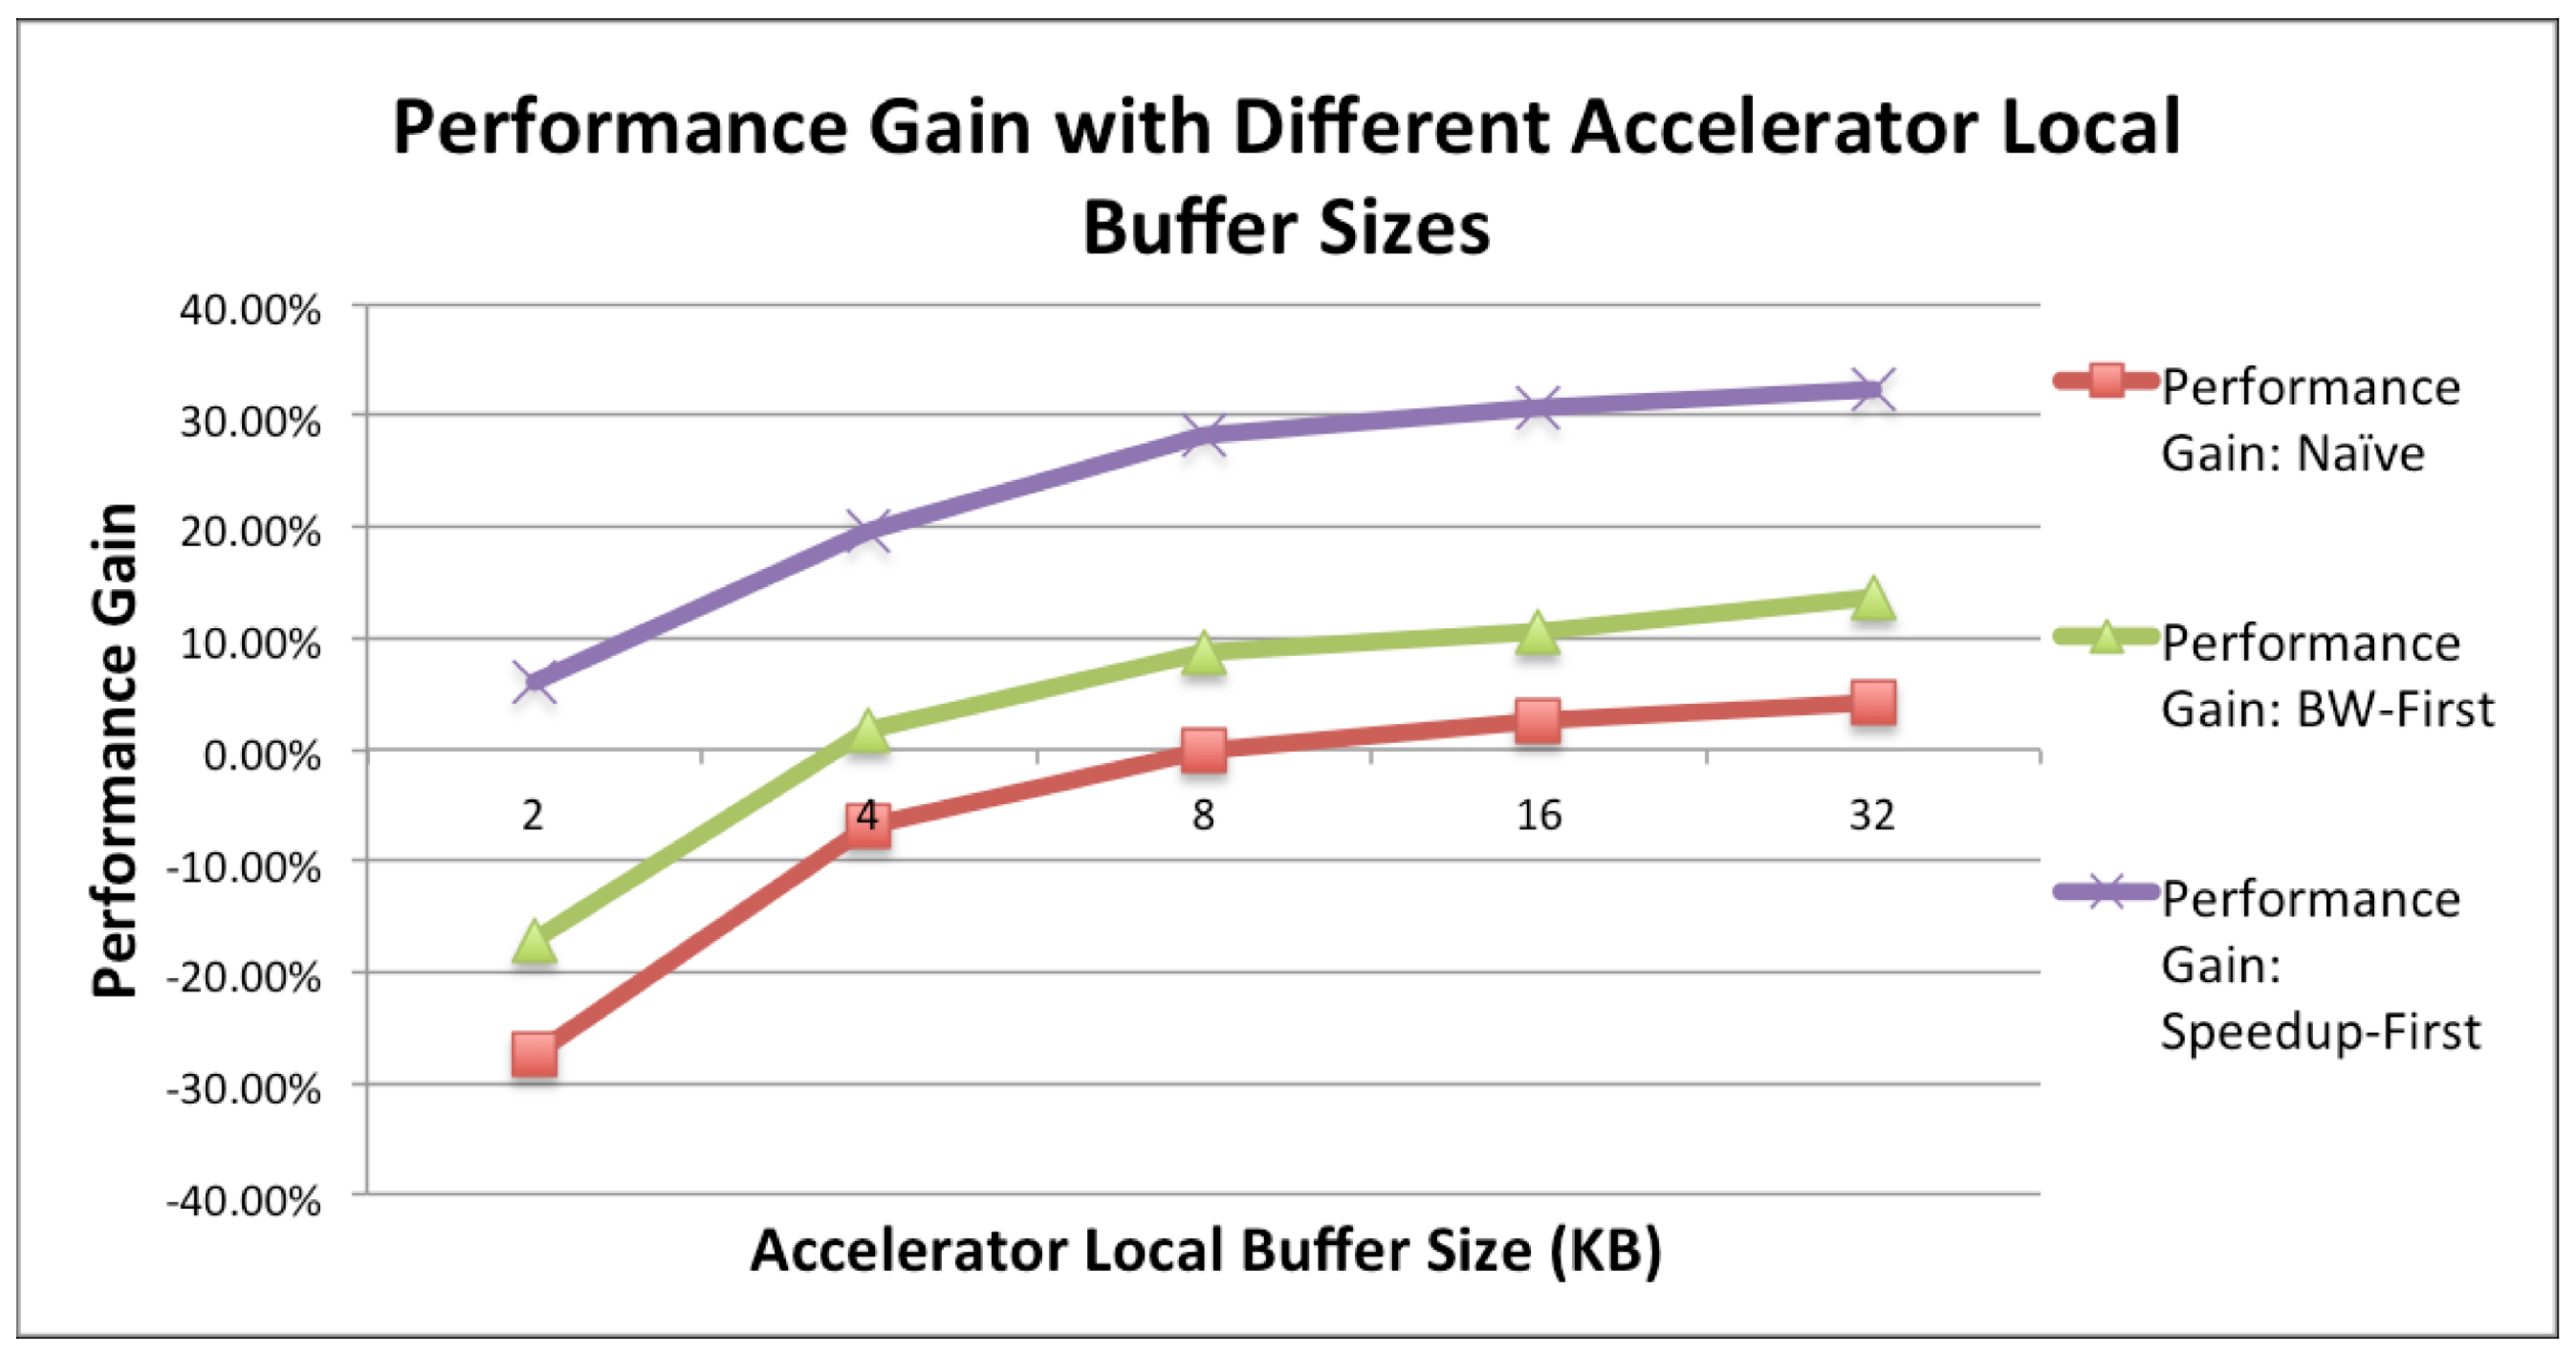
\includegraphics[width=4.5in]{Acc-Buffer-Performance}
    \caption{Performance Gain with Different Sizes of Accelerator Local Buffer.}
    \label{fig_acc_buffer_perf}
\end{figure}

\begin{figure}
    \centering
    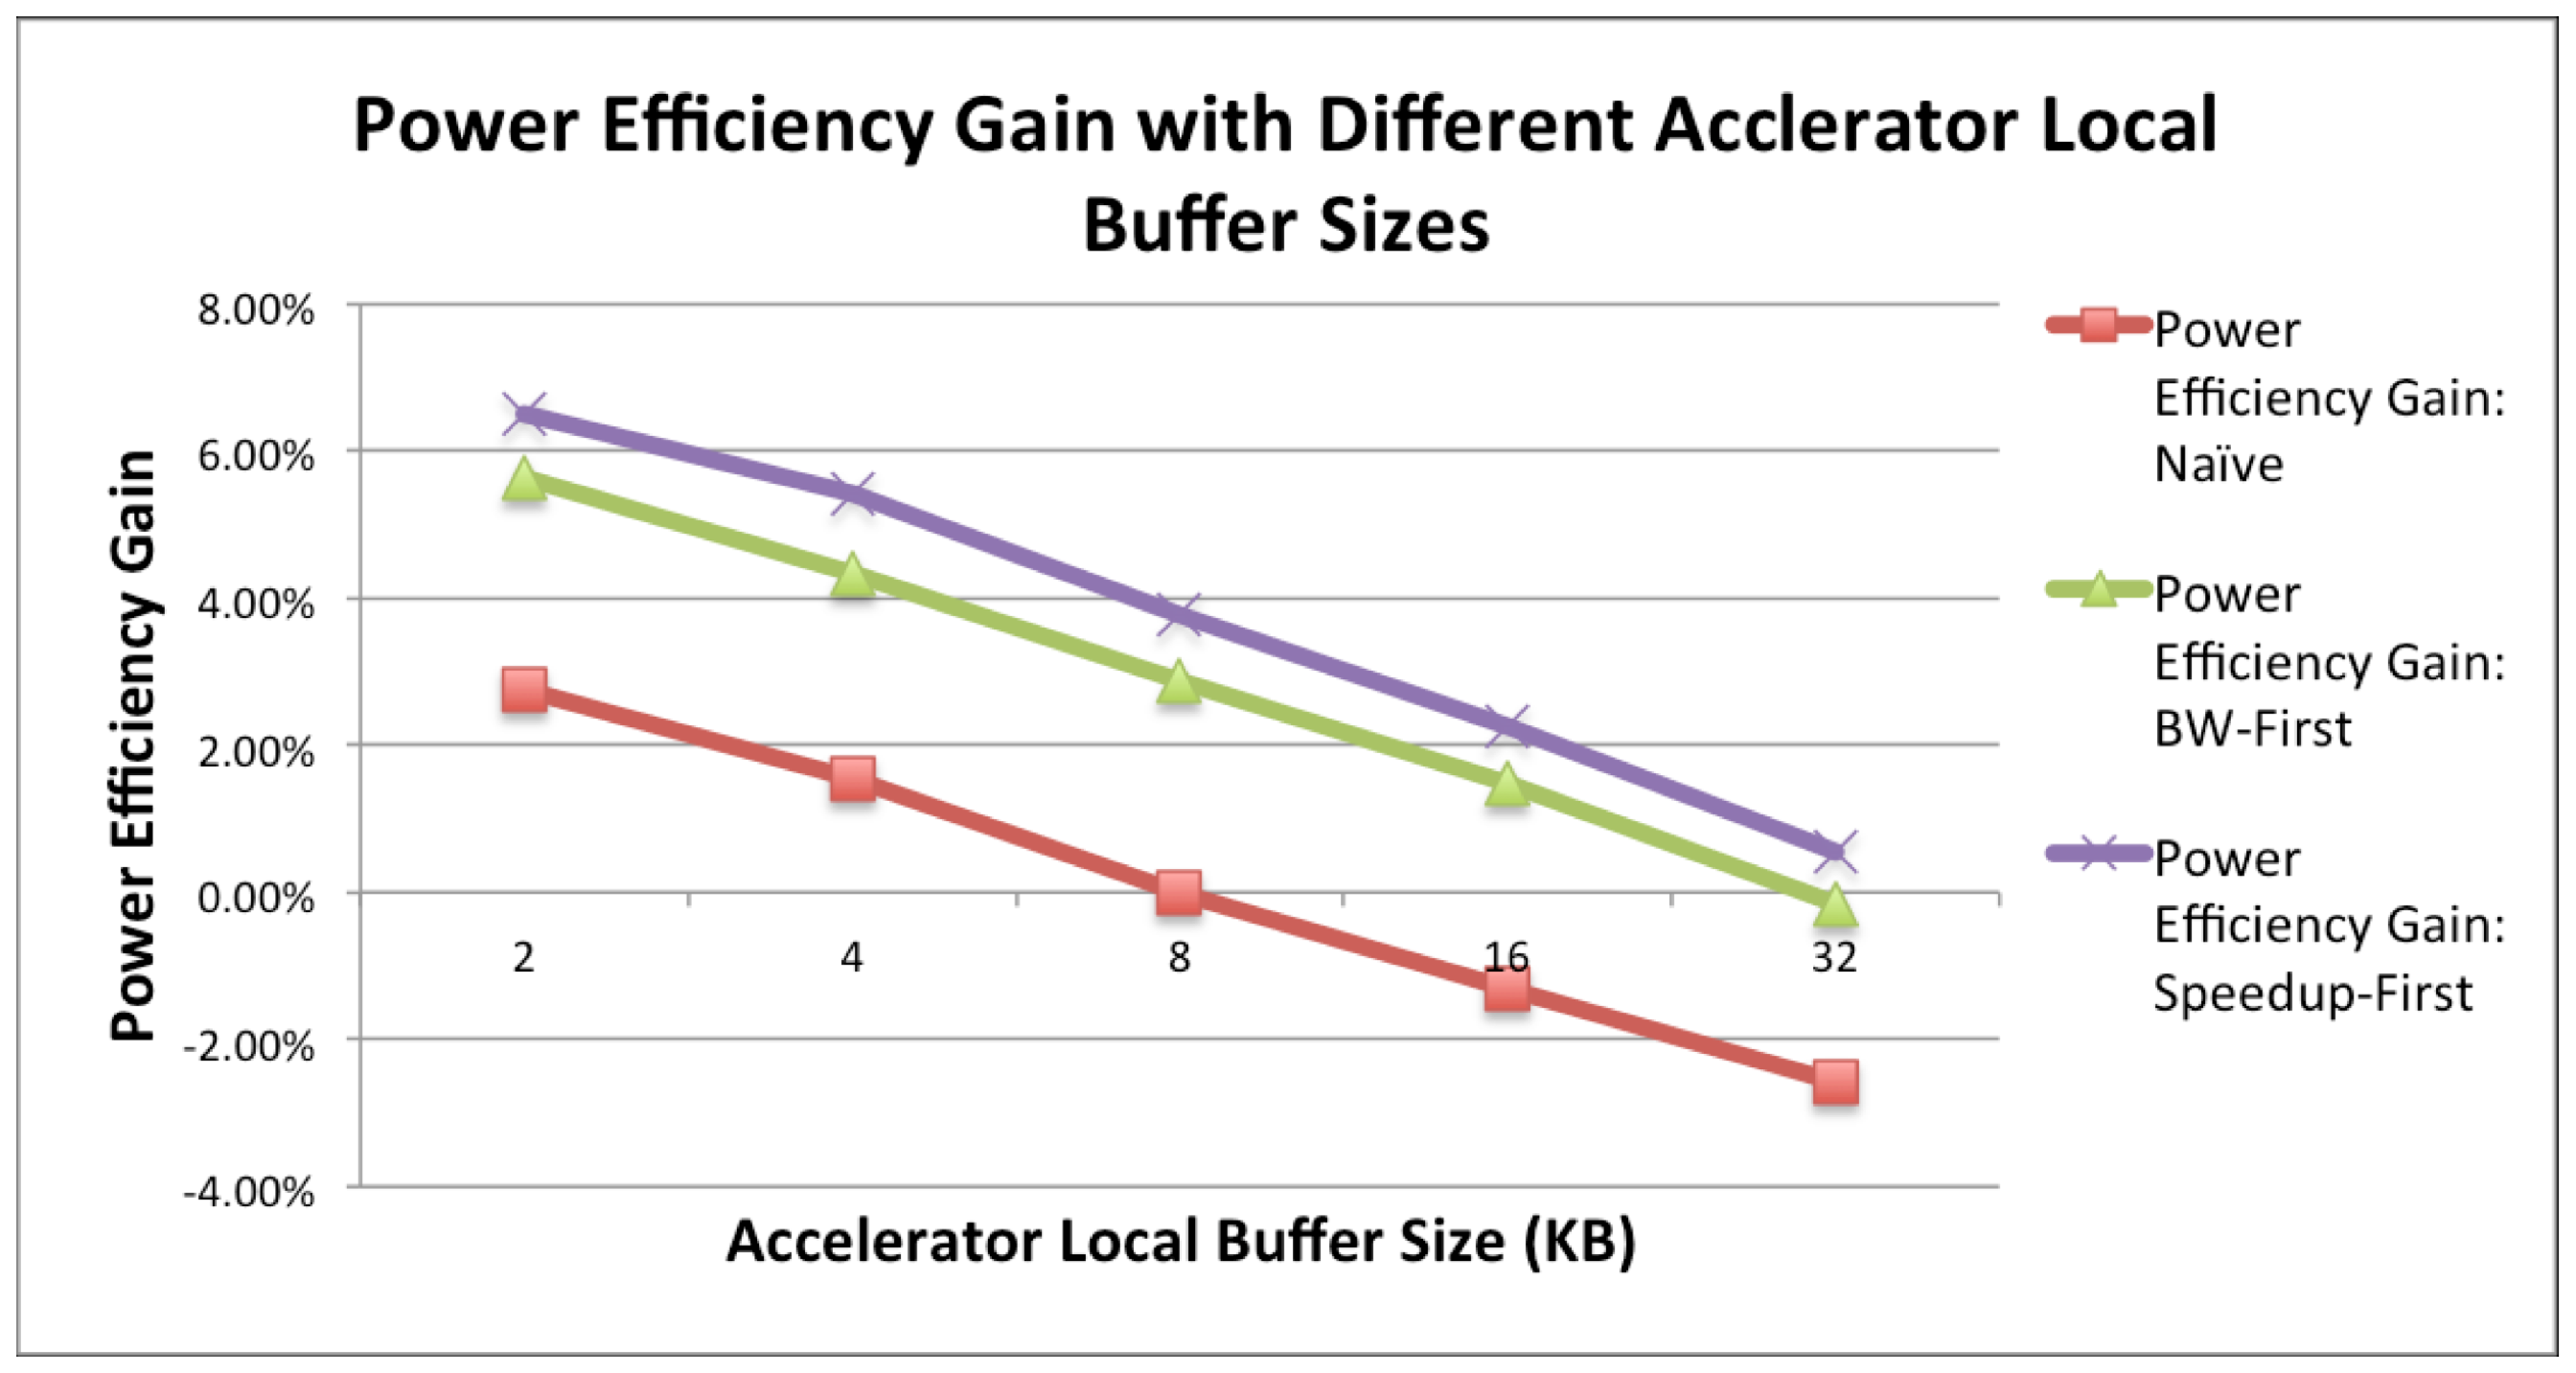
\includegraphics[width=4.5in]{Acc-Buffer-Power}
    \caption{Power Efficiency Gain with Different Sizes of Accelerator Local Buffer.}
    \label{fig_acc_buffer_power}
\end{figure}

\begin{figure}
    \centering
    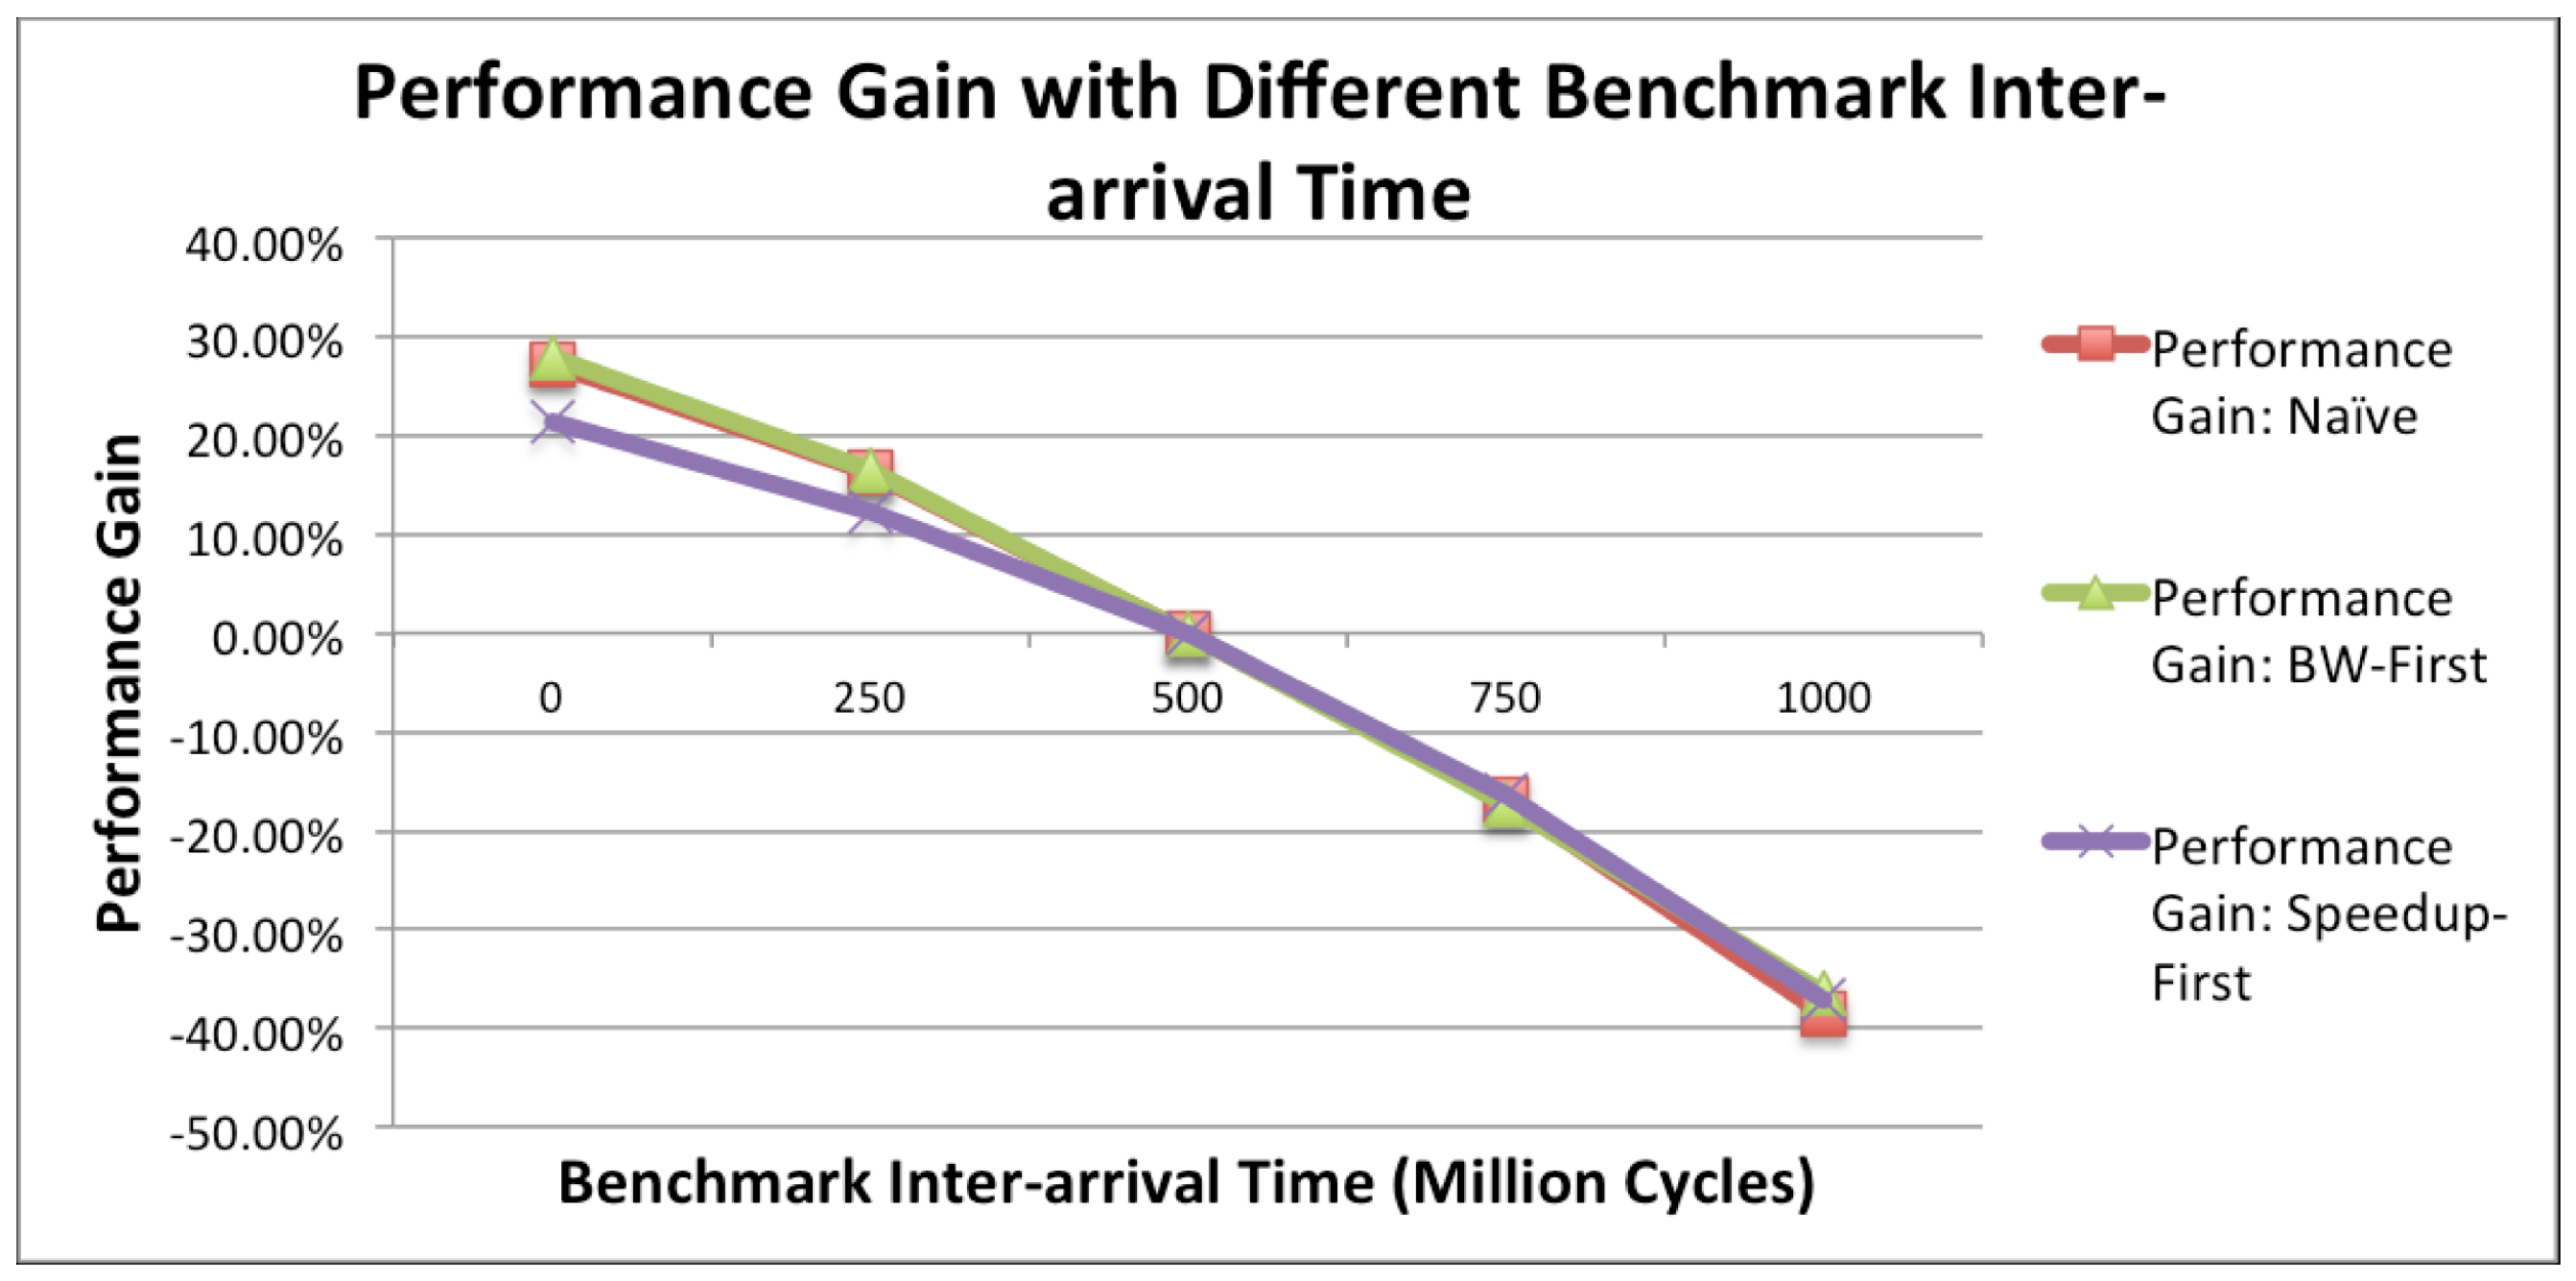
\includegraphics[width=4.5in]{Benchmark-Switching-Time}
    \caption{Performance Gain with Various Benchmark Inter-arrival Time.}
    \label{fig_benchmark-switching}
\end{figure}

\subsubsection{Utilization of Reconfigurable Resources}

Figure \ref{fig_acc_timeline} shows a sample of the run-time
reconfiguration process on the {\em Transformer}. The x axis is the
scheduling time window, and the y axis is the number of acceleration
functions instantiated on the SoC. Figure \ref{fig_acc_timeline}
reveals the dynamics of the workload and how {Transformer} adapts its
resources to demanding functions. Figure \ref{fig_logic_timeline}
illustrates how the utilization of various resources within the
reconfigurable logic changes over time.

Figure \ref{fig_acc_timeline}  also validates the advantages of run-time
configuration over fixed accelerators. We observe the maximum number of each
accelerators as: 3DES, SURF, Segmentation and Smithwaterman - 1
instantiation, IDSI and SLAM-J - 2 instantiations, SLAM-C and Jacobi -
3 instantiations. To achieve the same performance, the total logics we
would need if we rely on fixed onchip accelerators are: SLICE - 17848, FF
- 14511, LUT - 13192, BRAM - 255. That is, we would need at least 3.8 times
more SLICE and 12.75 times more BRAM to perform comparably as {\em Transformer}. 
This is a example for your.


\begin{figure}[ht]
    \centering
    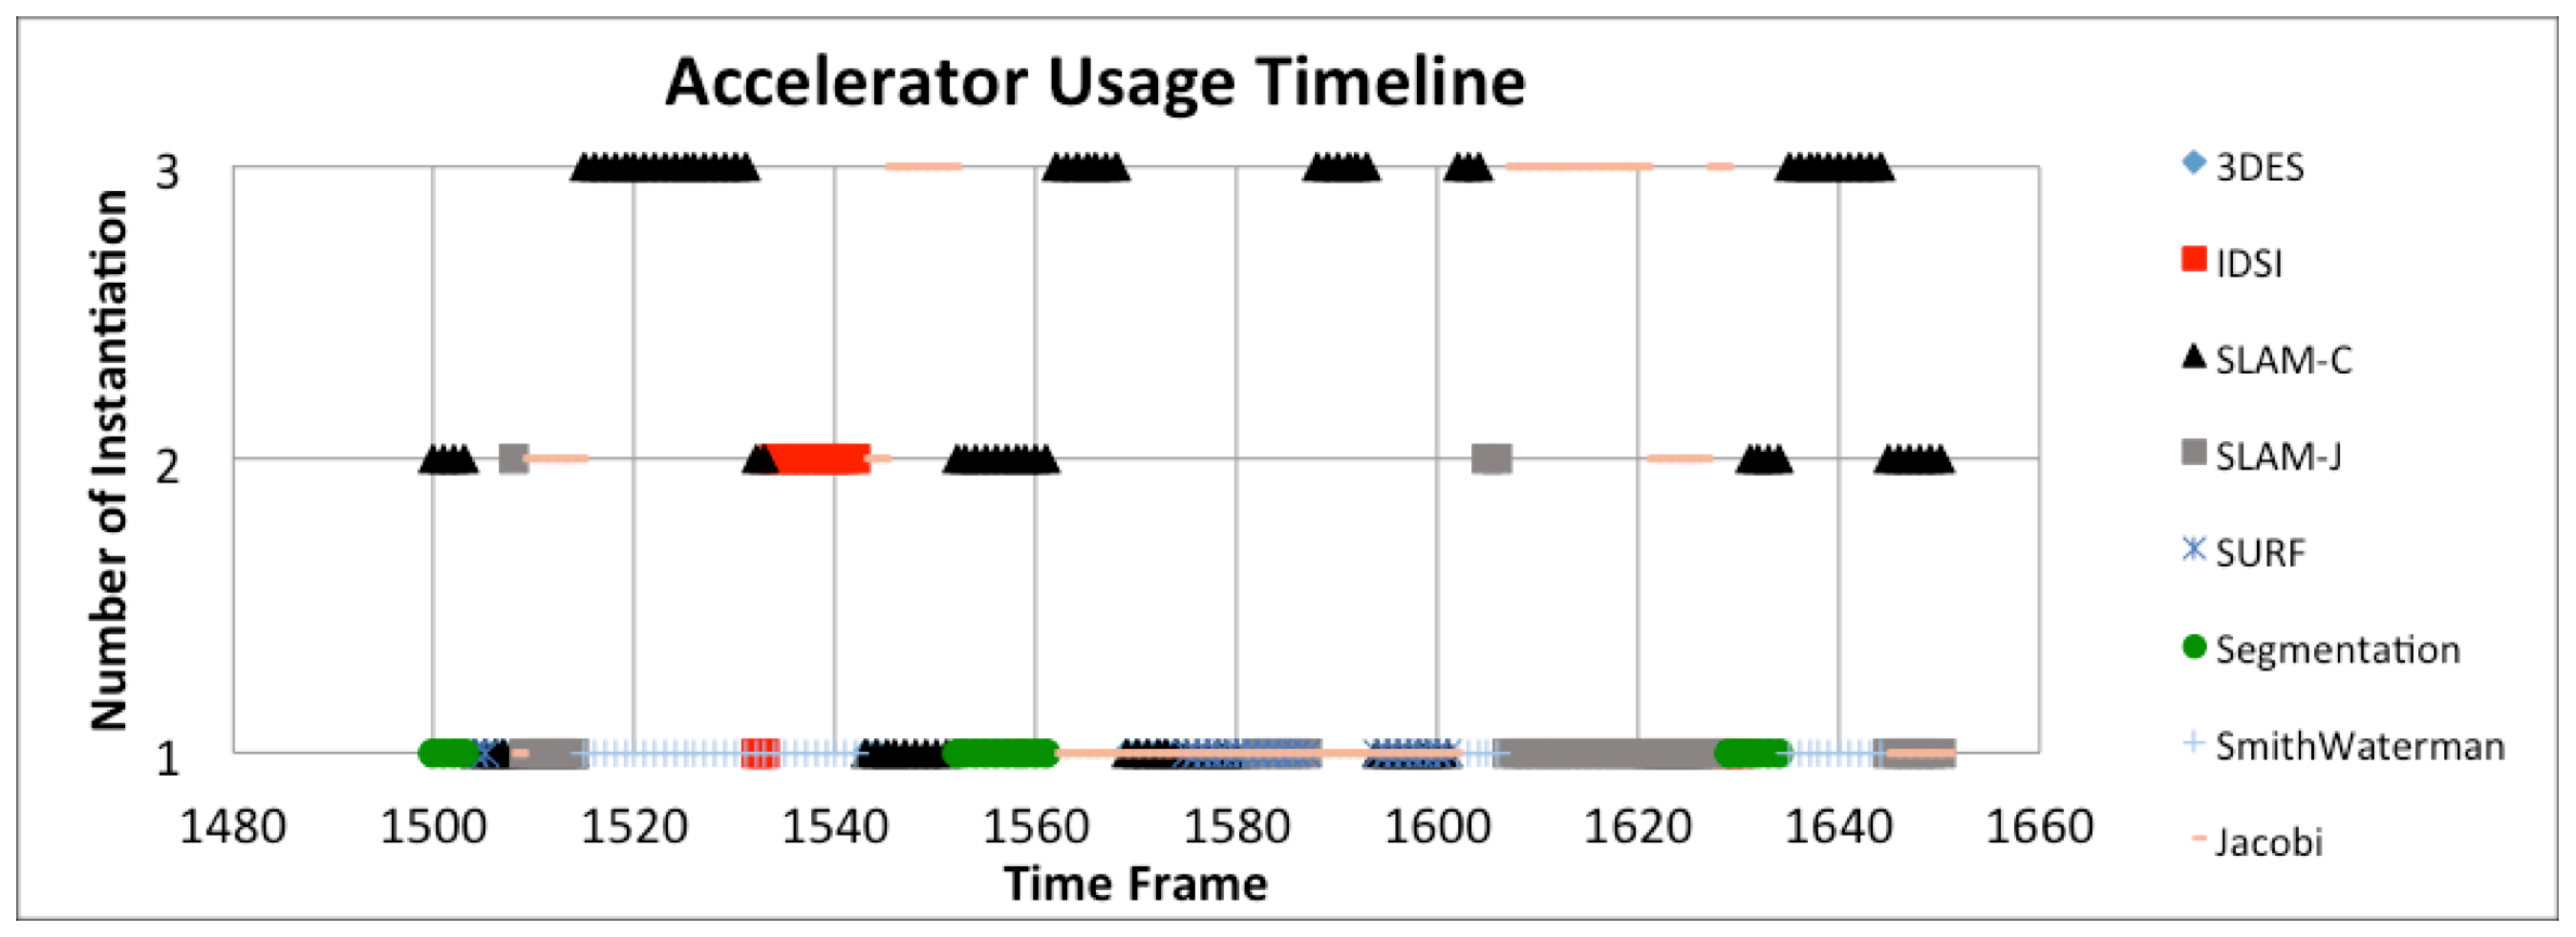
\includegraphics[width=6.0in]{Acc_timeline}
    \caption{Accelerator Usage Timeline.}
    \label{fig_acc_timeline}
\end{figure}

\begin{figure}[ht]
    \centering
    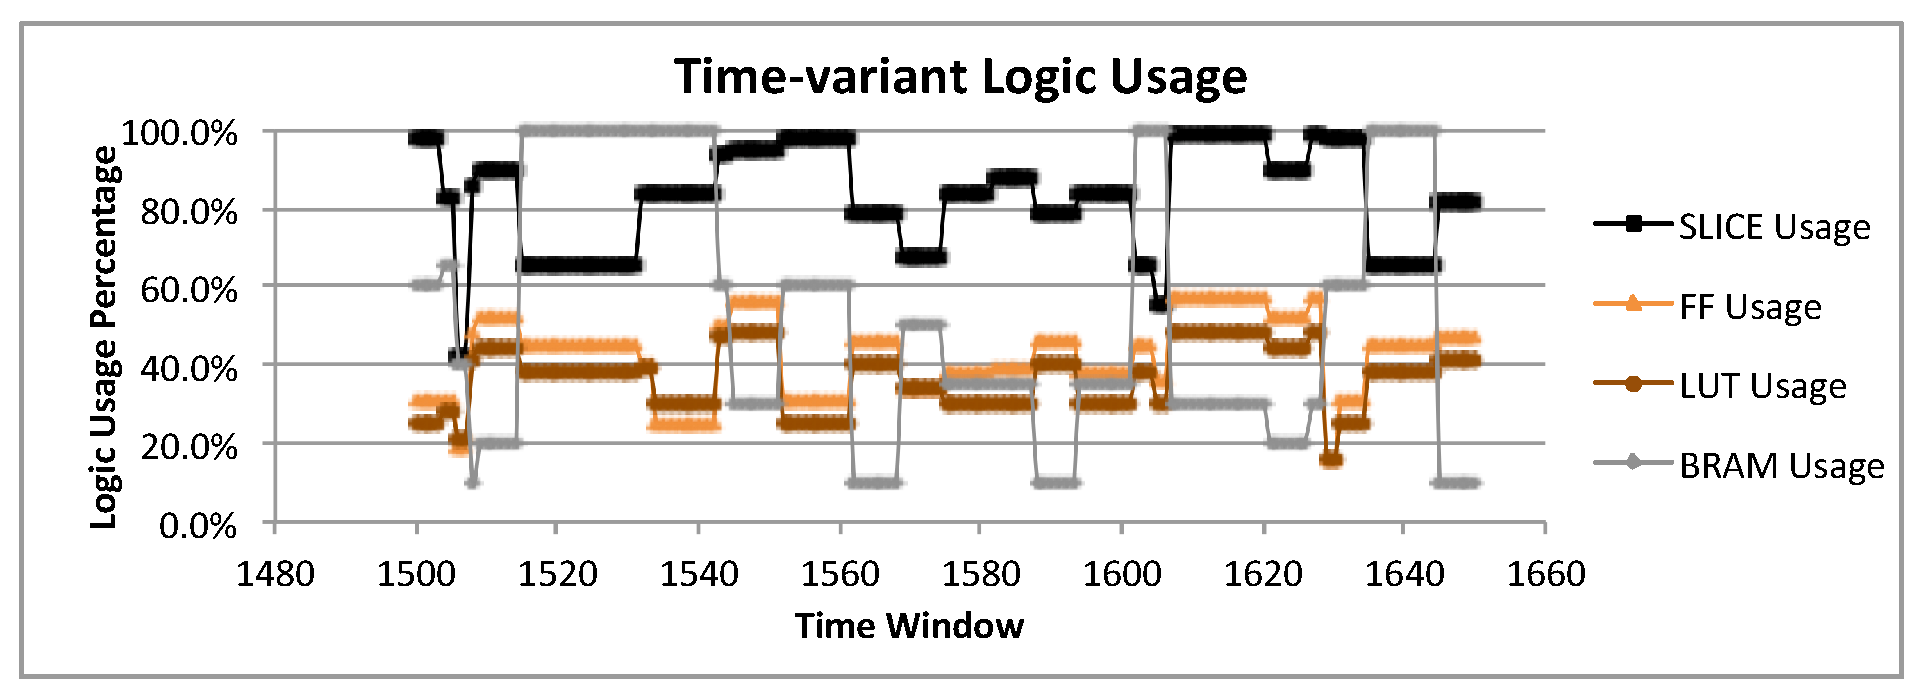
\includegraphics[width=6.0in]{Logic-Usage-Timeline}
    \caption{Total Logic Usage Timeline.}
    \label{fig_logic_timeline}
\end{figure}


\section{Conclusion}
\label{sec_concl}

In this paper, we propose a heterogeneous architecture {\em
  Transformer} with an on-chip, partial reconfigurable logic to
transparently accelerate dynamic unpredictable workloads.
Reconfiguration controller and middleware are introduced to trace the
run-time demands of the accelerator functions and invoke acceleration
path. We derive two scheduling algorithms based on solving Knapsack
problem to combine accelerators. We model the details of
accelerators in a modified Multi2sim simulator and evaluate the
performance and power efficiency of {\em Transformer} with synthetic
workloads from a wide range of domains. The performance and power
efficiency gains are shown to be significant. We study how the 
architectural parameters impact the system performance and power. We
investigate the chip area allocation to cores and accelerators, and make interesting observations on the optimal partition of resources. 

In the near future, we plan to explore finer granularity
of reconfigurable resources and accelerator-aware NoC to maximize the
performance of {\em Transformer}. We also plan to compare Transformer
with ASIC-based accelerators which require much effort in VLSI
implementations. A FPGA-based prototype (with soft cores and partial
reconfiguration) running real-world workloads obtained from cloud
servers is in the works.

%In this paper, we propose a hybrid architecture with both general
%purpose cores and reconfigurable logic accelerators for power
%efficient computing, which is critical in both cloud computing and
%mobile devices. We also outline a control scheme to reconfigure the
%accelerator at run time in response to the dynamics of the
%workloads. We simulate such architecture with Simics based full system
%simulator by porting benchmarks and designing a device driver for
%accessing the accelerator from user-level threads. Our experimentation
%results show the effectiveness of the reconfigurable logic based
%accelerator and the run-time reconfiguration. This 
%preliminary study encourages us to investigate the performance of the proposed hybrid
%architecture in virtualization environments. 
%%We also plan to optimize the run-time
%%reconfiguration schemes for higher speedup, for example, considering
%%not only the demand of a function, but also the speedup of
%%the accelerated functions.


\section{Acknowledgment}
\label{sec_ack}

This work is supported in part by the Intel Embedded University Program.



%-------------------------------------------------------------------------
\bibliographystyle{elsarticle-num}

\bibliography{reference}

\end{document}

